\documentclass[12pt]{third-rep}

\setcounter{tocdepth}{3}
\setcounter{secnumdepth}{3}
\usepackage{hyperref}
\usepackage{floatrow}
\usepackage{pdfpages}


\graphicspath{ {./images/} }
\usepackage{multirow}
\usepackage[justification=centering]{caption}


%% Any characters from a % to the end of line are comments.

%% The third-rep class and this starter kit were written by 
%% Graham Gough <graham@cs.man.ac.uk>
%% If you have any comments or questions regarding this document,
%% please post them to the local newsgroup man.cs.tex.

%% This skeleton report is organised as a master file called
%% report.tex which then includes files for individual parts including
%% abstract.tex, chapter1.tex, chapter2.tex, chapter3.tex and
%% appendix1.tex.  

%% The third-rep style is a locally created style based on the
%% standard LaTeX report style. If you really want to have a look at
%% it, its source can be found in
%% /usr/local/share/texmf/tex/latex/mancs/third-rep.cls
%%
%% More information about LaTeX in general and the local setup in
%% particular can be found on the web at 
%% http://csis.cs.manchester.ac.uk/software/contrib/latex
%%
%%%%%%%%%%%%%%%%%%%%%%%%%%%%%%%%%%%%%%%%%%%%%%%%%%%%%%%%%%%%%%%%%%%%%%%%
%%
%% This is an example of how you load extra packages.
%% Some packages are already loaded in the third-rep class

\usepackage{url} % typeset URL's sensibly

\usepackage{pslatex} % Use Postscript fonts

%% The best way to latex just one chapter is to uncomment lines such as
%% the next:
%\includeonly{chapter1}

%% This defines the title (the \\ forces a line break)
\title{A Universal Cellular Automata Simulator}
%% and author
\author{Rakha Djokosoetono}
%% and supervisor
\supervisor{Uli Sattler}
%% and the year of the report
\reportyear{2022}

%% this defines the file that contains the text of the abstract, there
%% must be one of these by the time you submit your report.
\abstractfile{abstract.tex}

%% this defines the file that contains the acknowledgements (it can be
%% omitted if you don't feel like thanking anyone
%% \thanksfile{merci.tex}

%% Uncomment the following lines if you want to include the date as a
%% header in draft versions. See the documentation for fancyhdr for
%% more ways of modifying headers (texdoc fancyhdr will show you the
%% docs) 

%\usepackage{fancyhdr}
%\pagestyle{fancy}
%\lhead{}  % left head
%\chead{Draft: \today} % centre head
%\lfoot{}
%\cfoot{\thepage}
%\rfoot{}

%% The following line sets up the use of PostScript fonts rather
%% than the standard bitmapped fonts.
\usepackage{pslatex}

%% Uncomment the following line if you want to change the name of the
%% Bibliography to References
%\renewcommand{\bibname}{References}

\usepackage{listings}

%% End of preamble, the actual document starts here
%%

\begin{document}

%% This actually creates the title and abstract pages
\dotitleandabstract

%% Generate contents etc
\tableofcontents
\listoffigures
\listoftables

%% These include the actual text
\chapter{Introduction}
\label{cha:intro}
\section{Motivation}
To simulate is the act of imitating real world processes or systems over time \cite{banks1996discrete}. It is also well understood that simulations are important in a myriad of contexts. In Science, Technology and Engineering subjects, simulations may be used for performance optimization or tuning, \cite{srinivasan2021words} or also ensuring systems provide acceptable levels of safetiness through the discipline of safety engineering \cite{verma2010reliability}. Simulations may also appear in scientific modelling of natural systems and economics \cite{orcutt1960simulation}. In general, however, simulations are used whenever the real system in question cannot be interfaced with (for whatever reason) \cite{srinivasan2021words}. 
\\ \\
One type of simulating is through the use of computer simulations. Simulating using computers started garnering popularity as far as World War II, when Jon Von Neumann and Stanislaw Ulam were investigating the complex behavior of neutrons during the Manhattan Project \cite{robeson}. Since then, simulations and modelling have undoubtedly become paramount in a variety of fields today, especially in dealing with complex systems.
\\ \\
Complex systems revolve around us - and oftentimes they can be generated by simple mechanisms \cite{southwell}. There are a handful of ways where such systems can be modelled using simple rules, but one such way of modelling complex systems can be done by cellular automata.
\\ \\
Commonly used as computer simulations, cellular automata (CA) is a discrete computation model studied in Automata Theory \cite{wolfram}. For  most simulations, CA would often appear as a grid of cells, with each cell in having one state from a finite set of states (e.g. \textit{on} state, or \textit{off} state). The states of these cells in the aforementioned grid may change each time-step (or generation), according to a set of transition rules and its neighbouring cells. 
\\ \\
CAs have demonstrated their simulation prowess in a variety of fields. They've oftentimes been applied to simulate systems in physics and biology \cite{wolfram}, forest fire propagation \cite{freire}, population dynamics \cite{mavroudi} \cite{moreno}, and can even be implemented in game development \cite{kowalski} among many others. Therefore, on the basis of the variety of a cellular automata's uses, this project's aim is to build a universal cellular automata simulator, where the user can define their own cellular automata rules in how the simulator would step. 
\section{Objectives}
\subsection{Objective 1: Research \& Development}
To achieve the aim of building a universal cellular automata simulator, background research is essential in understanding the underlying concepts of a cellular automata, its different types, and identify its various applications in addition to understanding what technologies are there to help me. The simulator should also allow the users to input their own rules in the simulation.
\\ \\
Therefore, an outline of my objectives in the scope of Research would be to:
\begin{itemize}
    \item gain a deeper understanding of cellular automata - understand what they are and different types of them, how they operate, their various applications, and how they are typically implemented in code
    \item hone and develop skills in JavaScript (JS) and HTML,
    \item browse various existing frameworks that might work as building blocks for the application
    \item come up with a rule format that is readable for humans
\end{itemize}
After research is done, then the goal will be to build a universal cellular automata simulator.
\subsection{Objective 2: Evaluation}
The final objective of the project is to evaluate the usefulness of this tool to the computer science university students and gather feedback on it. I define usefulness in this case as how easy the users can understand how to use the simulator. In particular, I'd like to obtain feedback on how easy to understand and use the rules are. Qualitative information will be gathered through small-scale interviews. 
\\ \\
The population of computer science students is chosen as the target audience. This is because the end product involves interfacing with text written in the JSON format, and of course cellular automata. The aforementioned group is therefore more likely to understand the JSON format and cellular automata.
\\ \\
Qualitative evaluation will be performed by short interviews where the user will use the system. Without the appropriate user feedback, the system's usability will forever remain subjective speculation to me, the developer. 
\chapter{Background Theory}

\section{Cellular Automata}
The meaning of \textit{cellular}, in this context, is "relating or consisting of living cells". On the other hand, the word \textit{automata} originates from the Greek language meaning "self-acting, self-willed, or self-moving". By combining the two words, the term Cellular Automata (henceforth CA) etymologically means living cells that move or act by its own willingness. As briefly touched upon in the previous section, CA are a grid of \textit{living} "cells", each cell pertaining to a particular "state". 
\\ \\
A CA consists of the following necessary components: the cells, states, neighbourhood type, and transition rules. Additionally, the term "generation" (pl. "generations") also need definition. Their meanings are as below:
\begin{itemize}
    \item \textbf{Cells}: The meaning of a cell in CA can be taken from its definition in biology, meaning the smallest, structural unit of an organism. In the context of CA in this project, this means it is the smallest unit of the grid. 
    \item \textbf{States}: In a CA, each cell has a state. Systems that  are \textit{stateful} means they are designed to remember preceding events \cite{harris2010digital}. In the context of CA, this information on preceding events is encapsulated in each cell's state, that may change depending on a certain set of \textit{transition rules} (see definition below). The \textit{state space} \label{state_space} is the set of states a system can occupy. As CAs are discrete models \cite{wolfram} 
    \item \textbf{Neighbours}: The neighbours of a cell are essentially cells that live in close proximity with the cell in question. There are different types of neighbourhoods, but in the context of this report, these neighbours can be defined simply as other cells that directly touch the cell in question (i.e. they are \textit{neighbouring}).
    \\ \\
    A more detailed description of this neighbourhood type can be found in section 2.1.3.
    \item \textbf{Transition Rules}: Transition rules are the rules that determine the next state of each cell with respect to the current state of the cell and the states in its neighbourhood. In most cellular automata, these are typically expressed as mathematical functions \cite{toffoli1987cellular}. Typically, these rules are applied to the entire CA grid simultaneously, though there are exceptions to how the rules are applied to a specific subset of CA \cite{schiff2011cellular}. These exceptions will not be discussed in this paper.
    \item \textbf{Generation}: A "generation" in a CA grid represents how many times the transition rules have been applied to each of the grid's cells. The initial state of a CA grid is represented at generation zero, (typically noted as generation time \textit{t} = 0). A new generation is therefore created by advancing \textit{t} by 1 (i.e. \textit{t} = \textit{t} + 1). This implies that the transition rules are applied once to the grid. Incrementing \textit{t} by integer \textit{n} will therefore apply the transition rules to the CA a number of \textit{n} times.
\end{itemize}
In retrospect, CA can be defined asa grid of "cells", where each cell has a "state", and in which those cells' states' evolve according to the a certain set of "transition rules". Cellular automata may operate in one, two, or more dimensions. However, the 2D variant will be the model implemented in this project. 

\subsection{Totalistic Cellular Automata}

Totalistic CAs are a special type of CAs, in the way that their state transition rules operate in a very specific manner. Extending the definition of transition rules from the section above, totalistic CAs have transition rules that determine the next state of each cell with respect to a certain number of states present in the cell in test's neighbourhood \cite{wolfram_2002}. An example of a totalistic CA is the game development map generation application (more on \ref{gamedevimp}).
\\ \\
If the transition rules in a totalistic CA also consider the state of the cell in test, then the CA can be labelled an \textit{outer} totalistic CA. \textit{Outer} totalistic CAs mean that the state of a cell at generation \textit{t} depends on both its own state, and the total of its neighbours both at generation \textit{t - 1} \cite{ilachinski_2002}. An example of an outer totalistic CA is Conway's Game of Life.
\\ \\
In essence, the only difference between a totalistic CA and an 
\textit{outer} totalistic CA is that the latter determines the next state of the cell while considering its current state as well.

\subsection{Probabilistic Cellular Automata}
Stochastic or Probabilistic cellular automata (henceforth PCA) outline the special state transition rules in a given CA. This means that instead of cells transitioning to a state based on the number of neighbours they have (and their states), each cell has a probability \textit{P} to transition to another state \cite{louis_nardi_2018}. This special transition rule is used for Forest Fire Propagation models, particularly the model implemented by Freire \cite{freire}, such that cells that are flammable have a certain probability of burning down. 

\newpage
\subsection{Moore Neighbourhoods} \label{moore_neighbourhoods}
The Moore-type Neighbourhood can be defined as a two-dimensional lattice. In a square grid, it contains the central cell and the eight immediate cells touching bordering it \cite{weisstein}. This type of neighbourhood is one of the two most common types of neighbourhoods in CA. It is visualized in the following figure:
\\
\begin{figure}[h]
    \caption{Moore Neighbourhood in a 2D Square Grid \cite{wolfram}}
    \centering
    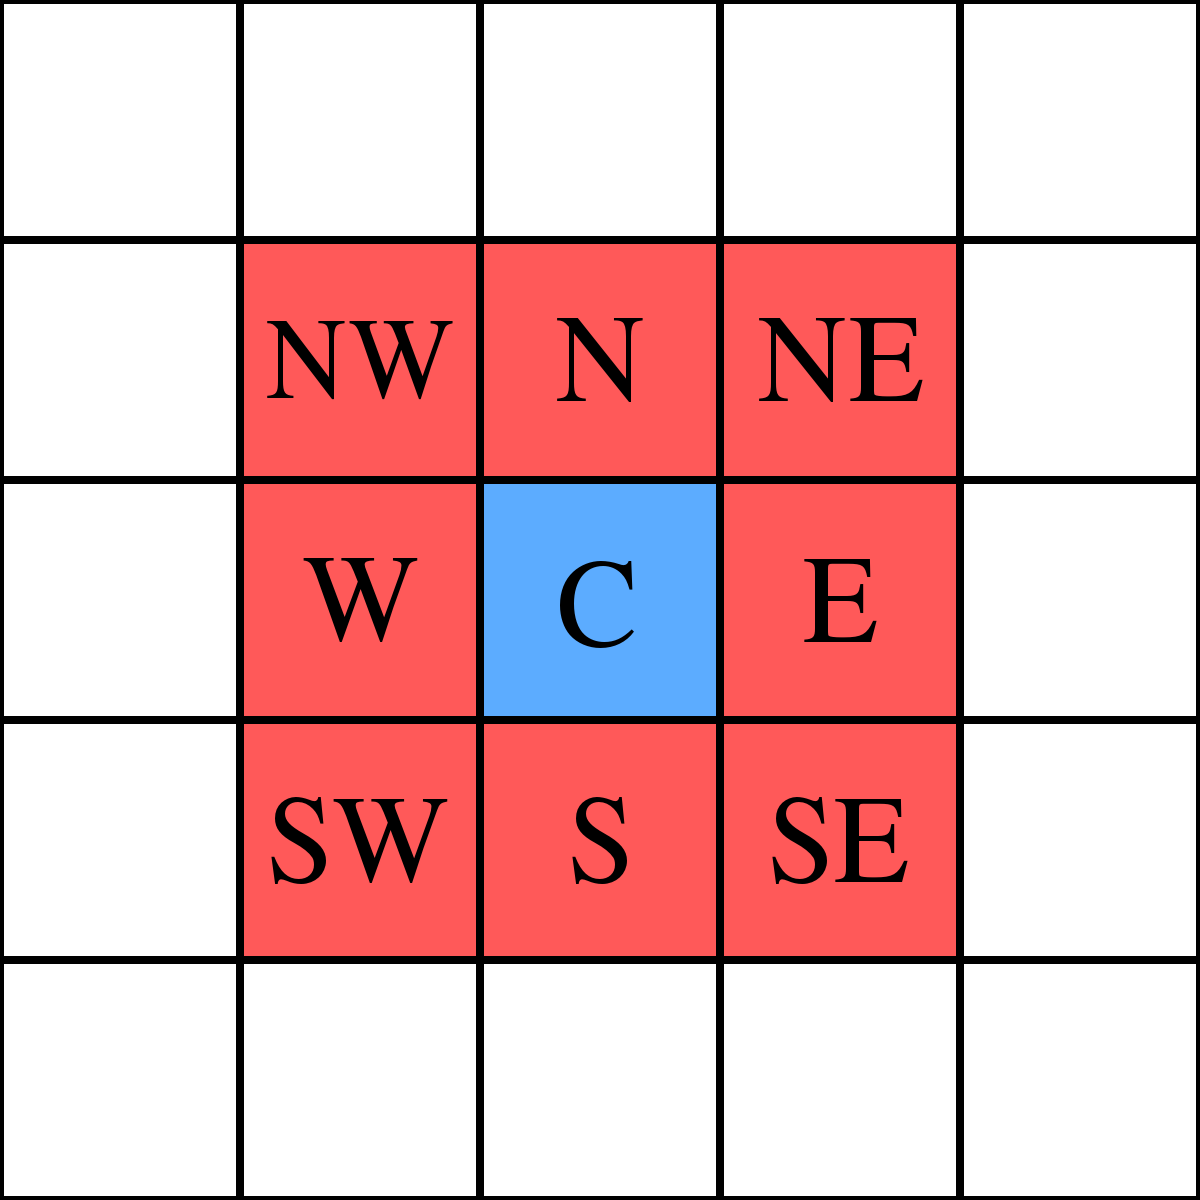
\includegraphics[scale=0.075]{moore_n.png}
\end{figure}
\\
Moore-type neighbourhoods can additionally consider a specific range or depth.
\begin{figure}[h]
    \caption{Moore Neighbourhood with Ranges \cite{wolfram}}
    \centering
    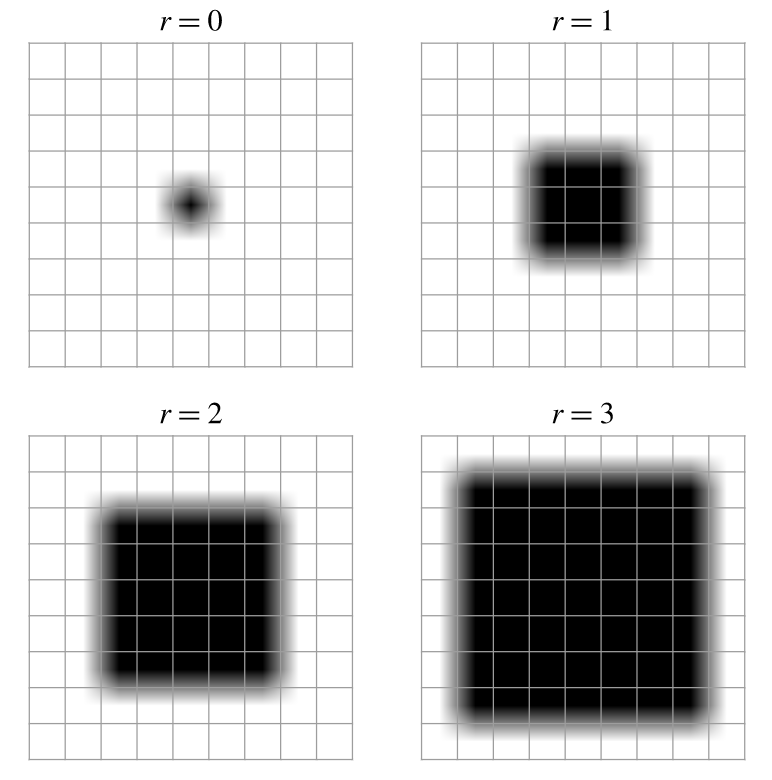
\includegraphics[scale=0.70]{moore_n_ranges.png}
\end{figure}
\\
\newpage
\section{Existing Applications of 2D Cellular Automata}
CAs have been implemented in a vast number of fields due to its reliance on relatively simple rules. These fields are briefly touched upon in the first chapter of this report. Furthermore, applying cellular automata on different areas of knowledge rely on manipulating the rules. This would suggest quite a substantial devation in rules when compared to conventional, more popular CAs such as Conway's Game of Life.

\subsection{Conway's Game of Life}
Conway's Game of Life (henceforth CGOL) is a two-state CA with a special set of transition rules. Developed by John Conway in 1970, CGOL is arguably the most popular two-dimensional cellular automaton \cite{gardner10fantastic}. It is an example of an outer totalistic CA. State transitions rely on Moore-type neighbourhoods, with deterministic rules. 
\\ \\
The state transition rules for each cell in a CGOL can be written in the form of if-statements:

\begin{itemize}
    \item \textbf{IF} the cell is \textit{alive} and has two or three live neighbours, \textbf{THEN} it remains alive in the next generation
    \item \textbf{IF} the cell is \textit{dead} and has exactly three live neighbours, \textbf{THEN} it becomes a live cell in the next generation
    \item \textbf{ELSE} the cell dies, or stays dead
\end{itemize}
Otherwise the following flowchart visualizes how the rules may work:
\begin{figure}[H]
    \caption{CGOL Rules Flowchart}
    \centering
    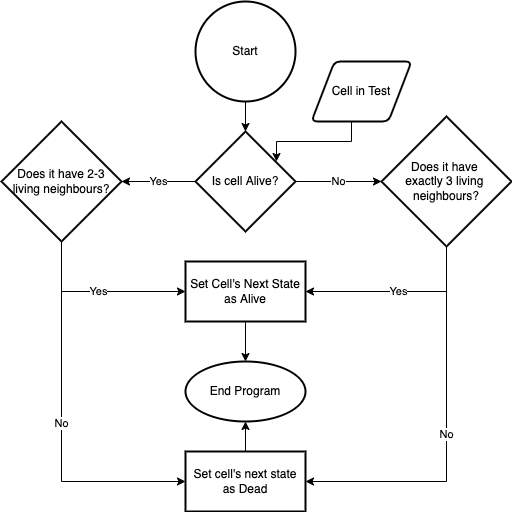
\includegraphics[scale=0.50]{flowchart_cgol.drawio.png}
\end{figure}
\noindent CGOL is Turing Complete. \cite{rendell2010simple}. The universality proof of CGOL in being Turing Complete was demonstrated by creating signals using the aforementioned Gliders, and combining them to create conventional logic gates (i.e. AND, OR, NOT) \cite{rendell2002turing}. 

\subsection{Forest Fire Propagation}
CAs have extensively been applied in forest fire propagation. Their models typically implement two-dimensional probabilistic cellular automata with three or more states. The CA model outlined by \cite{alexandridis_2011} make use of a square grid, with a potential of fire propagating to its eight nearest neighbours (i.e. Moore-type neighbourhoods). The rules according to the aforementioned journal are as follows:
\begin{enumerate}
    \item A cell that cannot be burnt stays the same
    \item A cell that is currently burning down will completely burn down at the next state
    \item A burned cell cannot burn again
    \item If a cell is currently burning, and its neighbours include cells containing vegetative fuel (i.e. 'burnable' state), then the fire can propagate to said neighbour with a certain probability. 
\end{enumerate}
The probability in this case may be affected by a myriad of factors. The article by Freire \cite{freire} has modelled propagation probabilities based on wind, slope shape, and vegetation density. 
\\ \\
The CA model outlined above, with probability functions integrated in its transition rules, is used to simulate the 2012 Algarve fire of Southern Portugal \cite{freire}. The same model, after a number of simulations, has also demonstrated an added value to assist in firefighting resource allocation in the event of a forest fire \cite{freire}.

\subsection{Population Dynamics}
In the study by Mavroudi \cite{mavroudi}, CAs were used to model population dynamics in the city of Salonica, Greece. Most CAs that are purposed to modelling population growth are mostly developed through trial and error (essentially heuristics) \cite{wu2002calibration}. In the context of city development, the rules in this CA are heavily influenced by its ecosystem. No city is regular, and these organic growths in population are usually affected by historical events and random decision making. \cite{batty1997cellular}. CAs have been used in urban population predictions since the late 1980s \cite{batty1999modeling}. 
\\ \\
Regarding urban growth and development, the CA rules are still a research topic \cite{batty1998urban}

\subsection{Game Development: 2D Map Generation} \label{gamedevimp}
Two-dimensional maps in games can often generated using CA. One of the CAs that can be used for map generationcan be a two-dimensional, two-state totalistic CA with deterministic state transition rules observing their Moore Neighbourhoods \cite{johnson2010cellular}. A common rule according to Johnson \cite{johnson2010cellular} for two-dimensional map generation is as such: 
\begin{itemize}
    \item \textbf{IF} a cell has more than four \texttt{wall} neighbours, \textbf{THEN} it turns to a \texttt{wall}
    \item \textbf{ELSE} the cell turns to a \texttt{floor}
\end{itemize}
\noindent The above is commonly used as cavern system generations in a game \cite{ashlock2015evolvable}. Another implementation of CAs in Game Development is a three-state genotype-to-phenotype based CA to recreate the Dune 2 Real-Time-Strategy map. In this implementation, however, the map is generated via genotype represented by matrices. CAs are only used here to create higher resolution maps through a stochastic process \cite{mahlmann2012spicing}. 

\section{Potentially Useful External Libraries and Tools}
To streamline the project development process, there are a number of libraries that may help as building blocks for the end product:

\subsection{JSON and JSON Schema} \label{json_schema}
JSON (short for JavaScript Object Notation) is a common data interchange format. JSON can contain JSON entities on its own, and is easy for humans to write, and computers to parse \cite{bassett2015introduction}.
\\ \\
JSON Schema on the other hand is a special type of JSON that can be used to validate whether another JSON meets the requirements specified on the schema. It is a schema language. Validators typically validate JSON entities against a schema that is supplied, such as in a MongoDB database instance or API requests \cite{pezoa2016foundations}.
\\ \\
Essentially, JSON Schema is a response to the lack of standardized metadata or schema language for JSON - the most popular data format for API requests and responses. However, this is still under research and development \cite{pezoa2016foundations}. 

\subsection{P5JS} \label{p5js}
P5JS is a JavaScript library, utilized for ’creative coding’. This library is targeted primarily for audiences with an intent to draw, and therefore a myriad of its keywords rotate on the concept of sketching and drawing on a canvas \cite{mccarthy2015p5js}. This library may be useful in visualizing the CA.

\subsection{TV4} \label{tv4}
Tiny Validator 4 (TV4) is a JS library written for use with JS or HTML/JS applications (typical installation using NPM or Yarn) \cite{tv4}. This library enables the use of JSON validation with a specified JSON Schema. If there were a validator component in the project, this library will surely prove useful. 

\subsection{Git, GitHub and GitHub pages}
Every step of the development process is synchronized with GitHub version control. Proper workflow is maintained to the best of my abilities, and this has made the development process easier. The final project is hosted on GitHub pages for everyone to see and to provide room for evaluation, using a custom subdomain purchased from Namecheap. The project can be found at \texttt{https://projects.rakhadjo.me/y3-project}
\chapter{Planning and System Design}

\section{Planning and Work Management}
The project was synchronized with GitHub version control from the very beginning. GitHub issues were used to keep track of features that are to be implemented in the project, in addition to patches and fixes. 
\begin{figure}[h]
    \caption{GitHub Issues for Tasks Tracking}
    \centering
    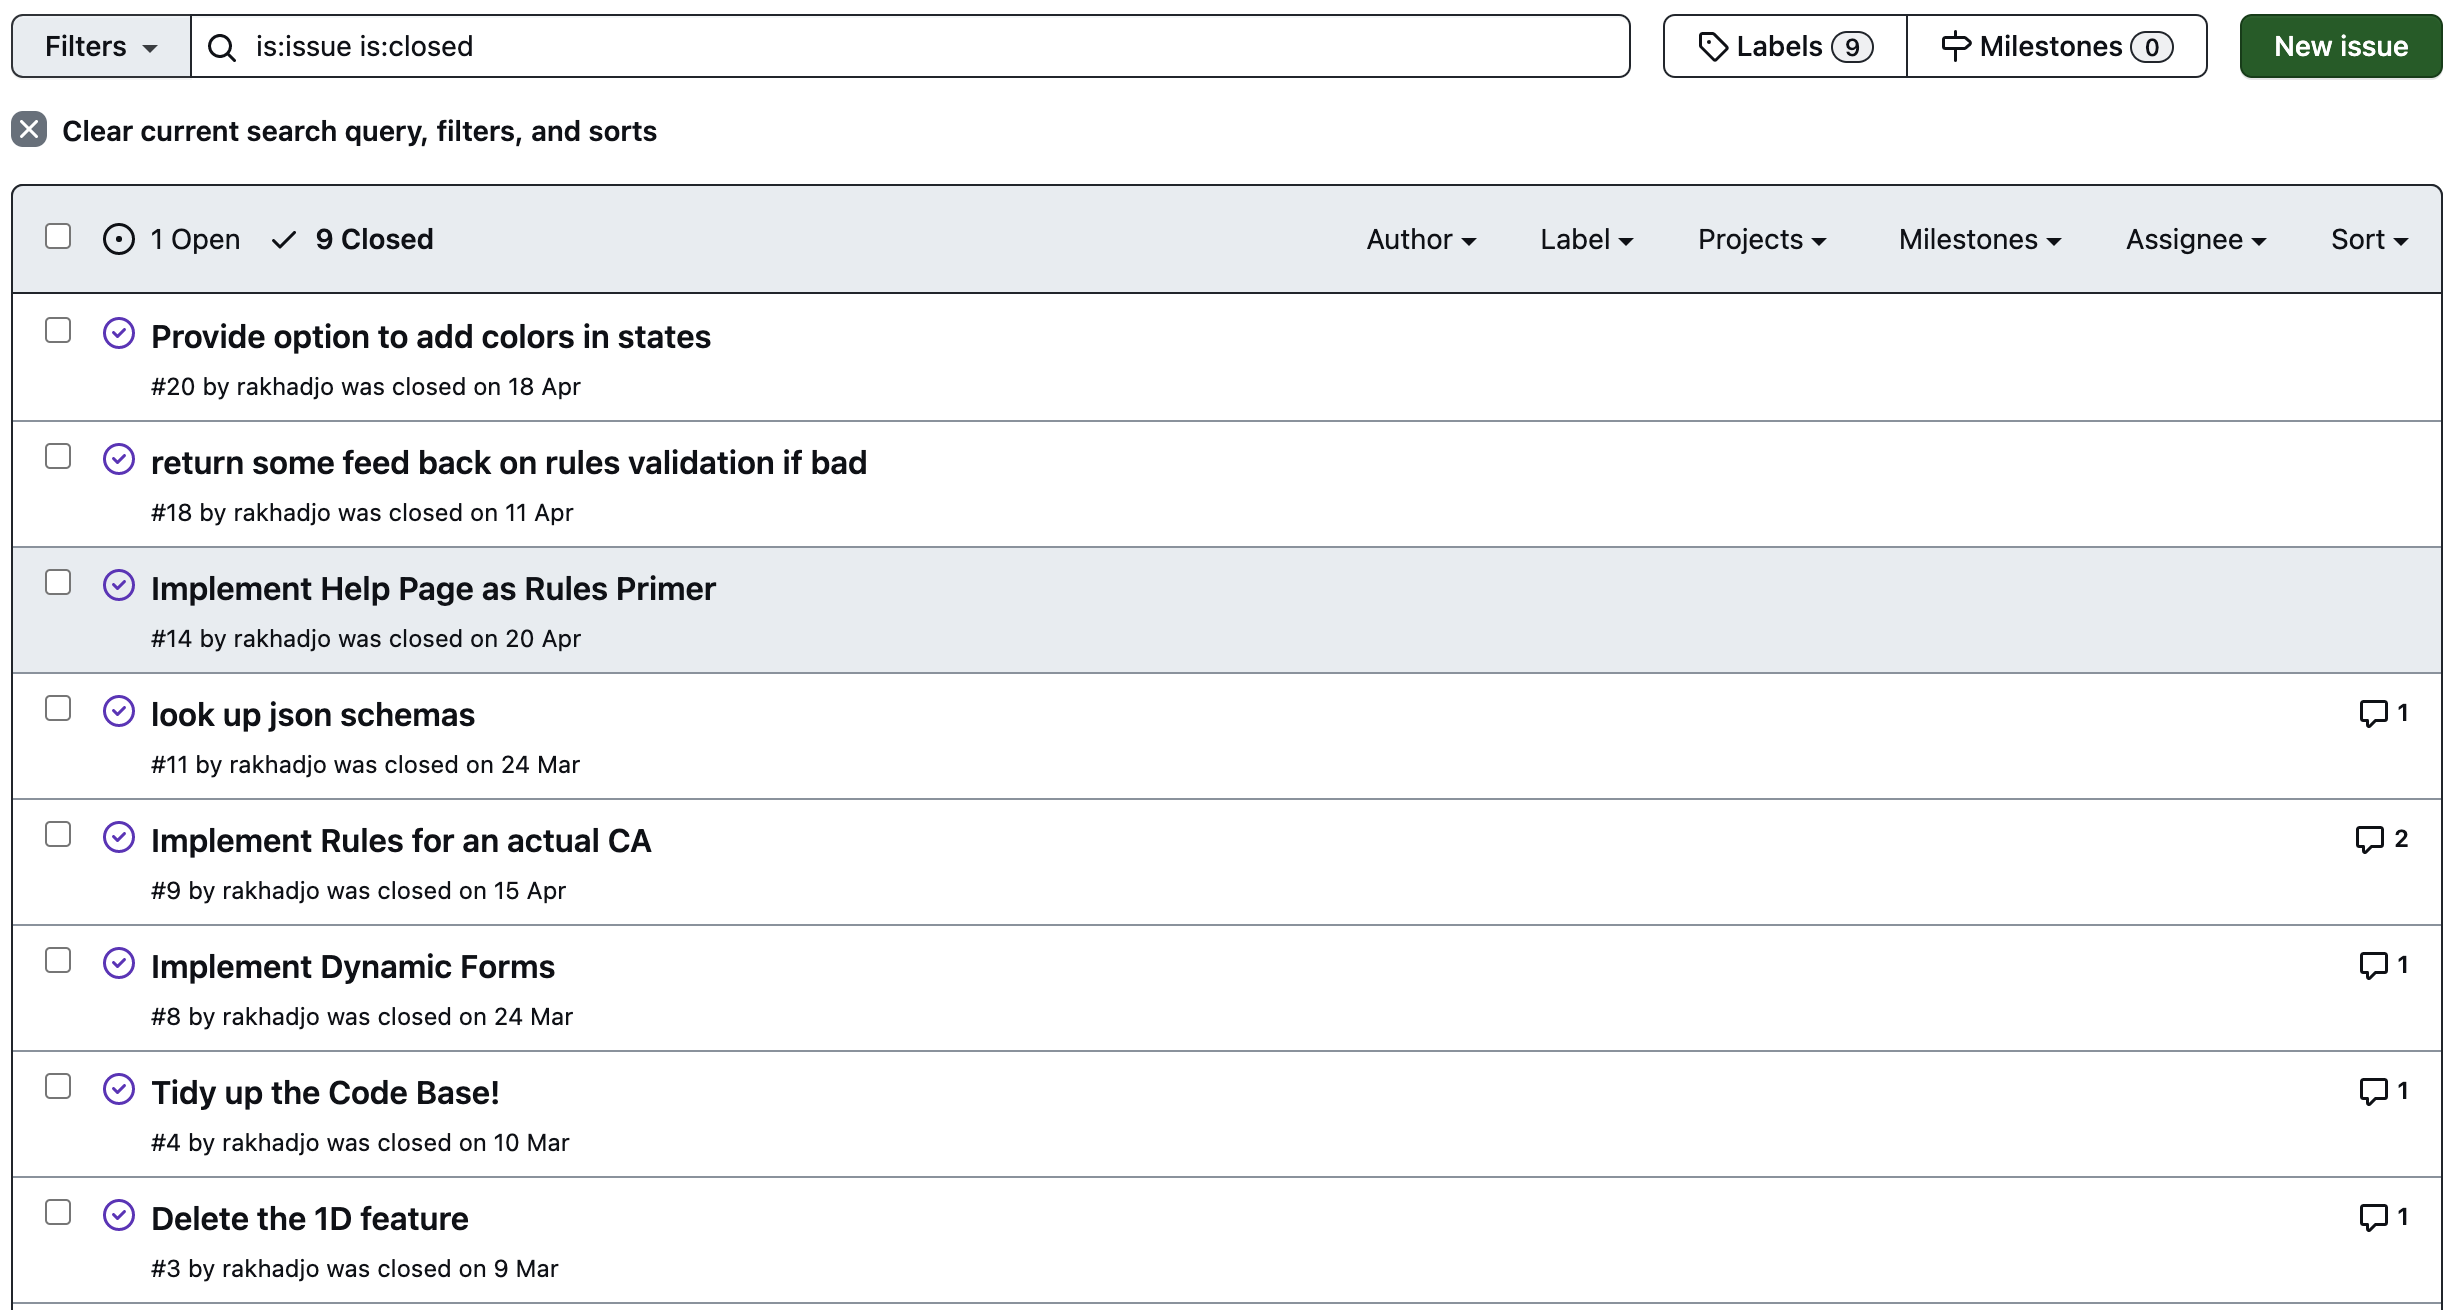
\includegraphics[scale=0.20]{github_issues.png}
\end{figure}
\\ 
Each issue calls for its own feature branch, and each feature is then integrated by merging pull requests from their respective branches to the \texttt{development} branch. \\
\begin{figure}[h]
    \caption{GitHub Pull Requests for Feature Merging}
    \centering
    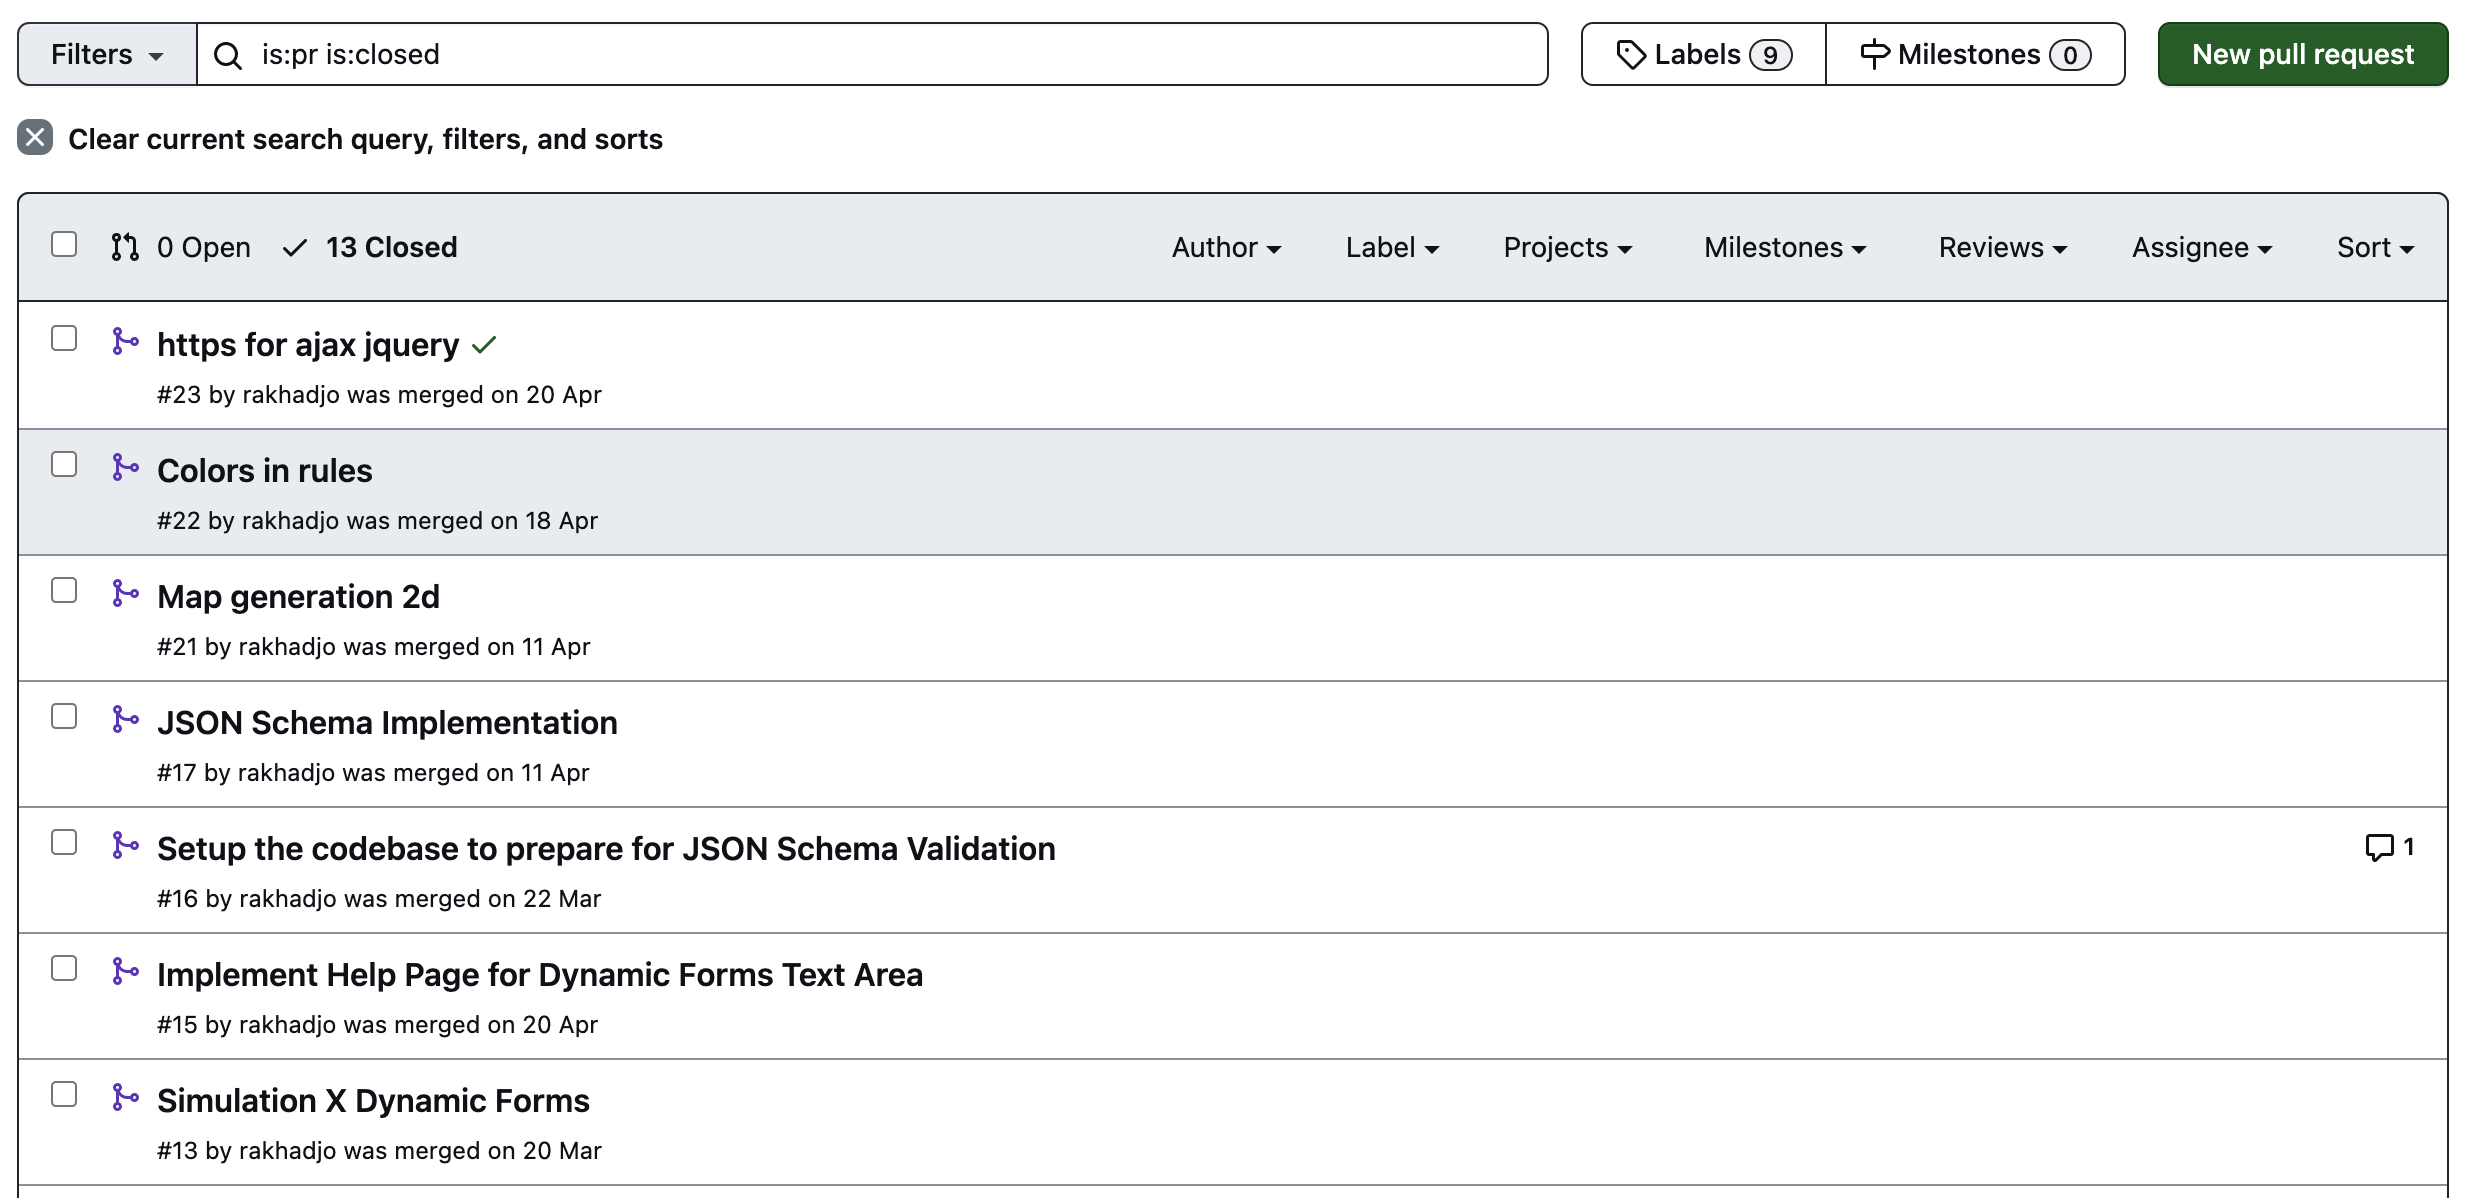
\includegraphics[scale=0.20]{github_prs.png}
\end{figure}
\\ 
A pull request to the \texttt{master} branch from the aforementioned \texttt{development} branch is opened from the very beginning, and merged upon the code freeze for submission.

\section{Features}
The main idea is to create a user interface which should be usable by university students in computer science, with some exposure to Cellular Automata. Note that this project does not aim to introduce the concept of cellular automata to its users. This means that provided the idea of cellular automata and a brief overview of how to use the rules, the user should be able to manipulate the rules and use the simulator.

\subsection{Functional Requirements}
Functional requirements outline the bare minimum as to how the system should behave. This project requires the system to, at the bare minimum and for all kinds of CAs:
\begin{itemize}
    \item \textbf{Graphical User Interface}: The GUI will take inspiration from an IDE, and be as ergonomic as possible.
    \item \textbf{Modify the CA rules}: Editable through the Rule Editor on the left hand side of the GUI. 
    \item \textbf{Change any of the state's colors}: This will be done by modifying the rules' contents in the \texttt{\$\_meta} tag, for preference or real-world visualization.
    \item \textbf{Change the CA rules}: Using the rules' contents from the text editor. 
    \item \textbf{Parse and Validate JSON Rules}: Potentially TV4/JSON Schema implementation.
    \item \textbf{Count Neighbours of Each Individual Cell}: CAs determine next state based on neighbour's states. 
    \item \textbf{Determine next state}: Provided the rules and the neighbour stats. 
\end{itemize}

\subsection{Non-Functional Features}
Non-functional features outline how the system is meant to behave, while describing its limits in its functionality. In the context of this project, the non-functional features are as follows:
\begin{itemize}
    \item \textbf{24/7 Availability}: Hosted on an always-on system.
    \item \textbf{Platform Independence}: Hosted on GitHub Pages, accessible and usable to everyone on the internet.
\end{itemize}

\section{Language Selection}
Due to the time constraint in the project, the final software was written in HTML and JavaScript. This allows the project to be instantly deployed as a static web page during testing, in addition to providing instant availability to the project only through a web browser without any unnecessary downloads.
\\ \\
Java and JavaFX was considered at one point, but JavaFX support online was relatively minimal. Additionally, different versions Java installations wouldn't have given the final project the same level of flexibility in deployment. Installation would therefore be impractical. 
\\ \\
Despite the tech stack being entirely front-end, I am defining the term "front end" as code that functions to change the user interface, and "back end" as code whose functions are not directly seen.

\section{Architectural Diagram}
As the details of each components and micro-components are discussed in the sections following, the below diagram represents the general architectural flow, alongside the names of the components. 
\begin{figure}[H]
    \caption{Architectural Diagram}
    \centering
    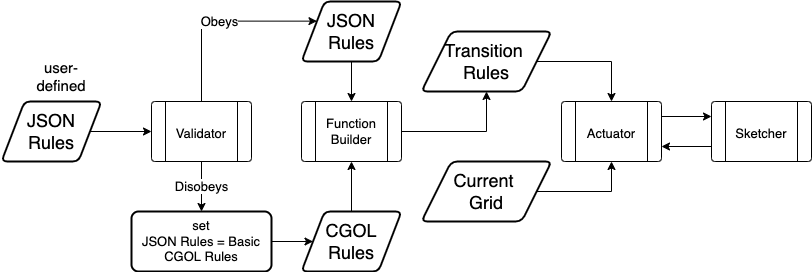
\includegraphics[scale=0.5]{arch.png}
\end{figure}
\noindent It is important to note that the validator, function builder, actuator and sketcher components are displayed as 'predefined', because its implementation will be shown here soon. 
\\ \\
Some components are not present in the diagram. That is because the dynamic rules format are somewhat related to the Validator, and the GUI overarches everything. 

\section{Architectural Components and Implementation}
The following subsections outline the different components working in tandem to fulfill the described features above, and justifying the decisions that were made. Additionally, the final implementation of each components are described in this section.

\subsection{Graphical User Interface (GUI)} \label{gui_component}
The GUI is designed to hold three main components to the system: the CA simulator, the rules editor, and the control buttons. An early sketch of the GUI is provided below: 
\\
\begin{figure}[H]
    \caption{Early GUI Sketch}
    \centering
    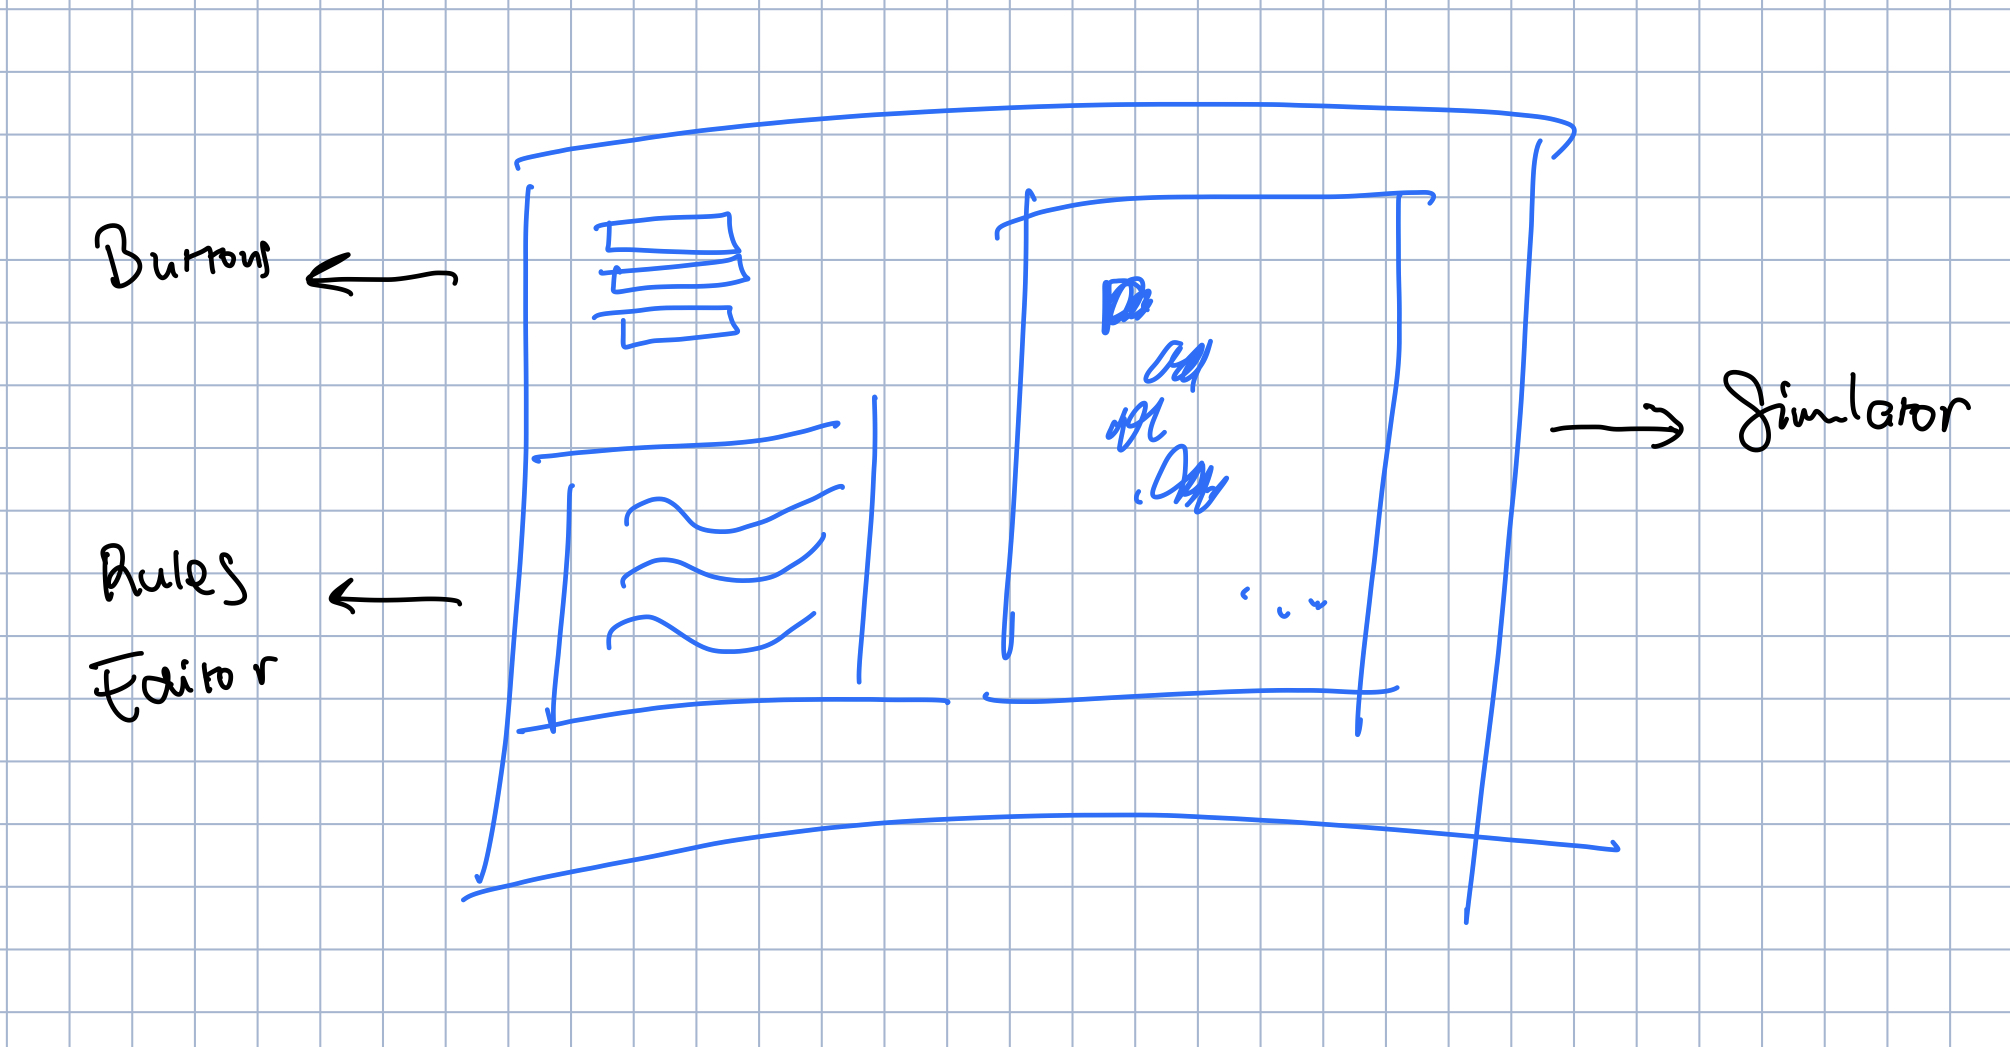
\includegraphics[scale=0.20]{early_ui_mockup.jpeg}
\end{figure}

\noindent The rules editor and buttons are to be positioned on the left side of the screen, whereas the simulator is placed on the right hand side. This design is inspired by a variety of IDEs, where buttons are typically placed on top of the editor area, and the output (in this case the simulator) is positioned on the right (oftentimes bottom). The choice of inspiration from an IDE is that the intended audience (for evaluation) of this project is Computer Science Students. There is a higher chance that the audience has interfaced with an IDE before, and my hypothesis is that this design will increase usability. This IDE-inspired design hopes to be ergonomic by adopting the principle of humans reading from left to right, up to down.
\\ \\
The final GUI is shown in the following:
\\
\begin{figure}[h]
    \caption{Final GUI Design}
    \label{fig:final_gui}
    \centering
    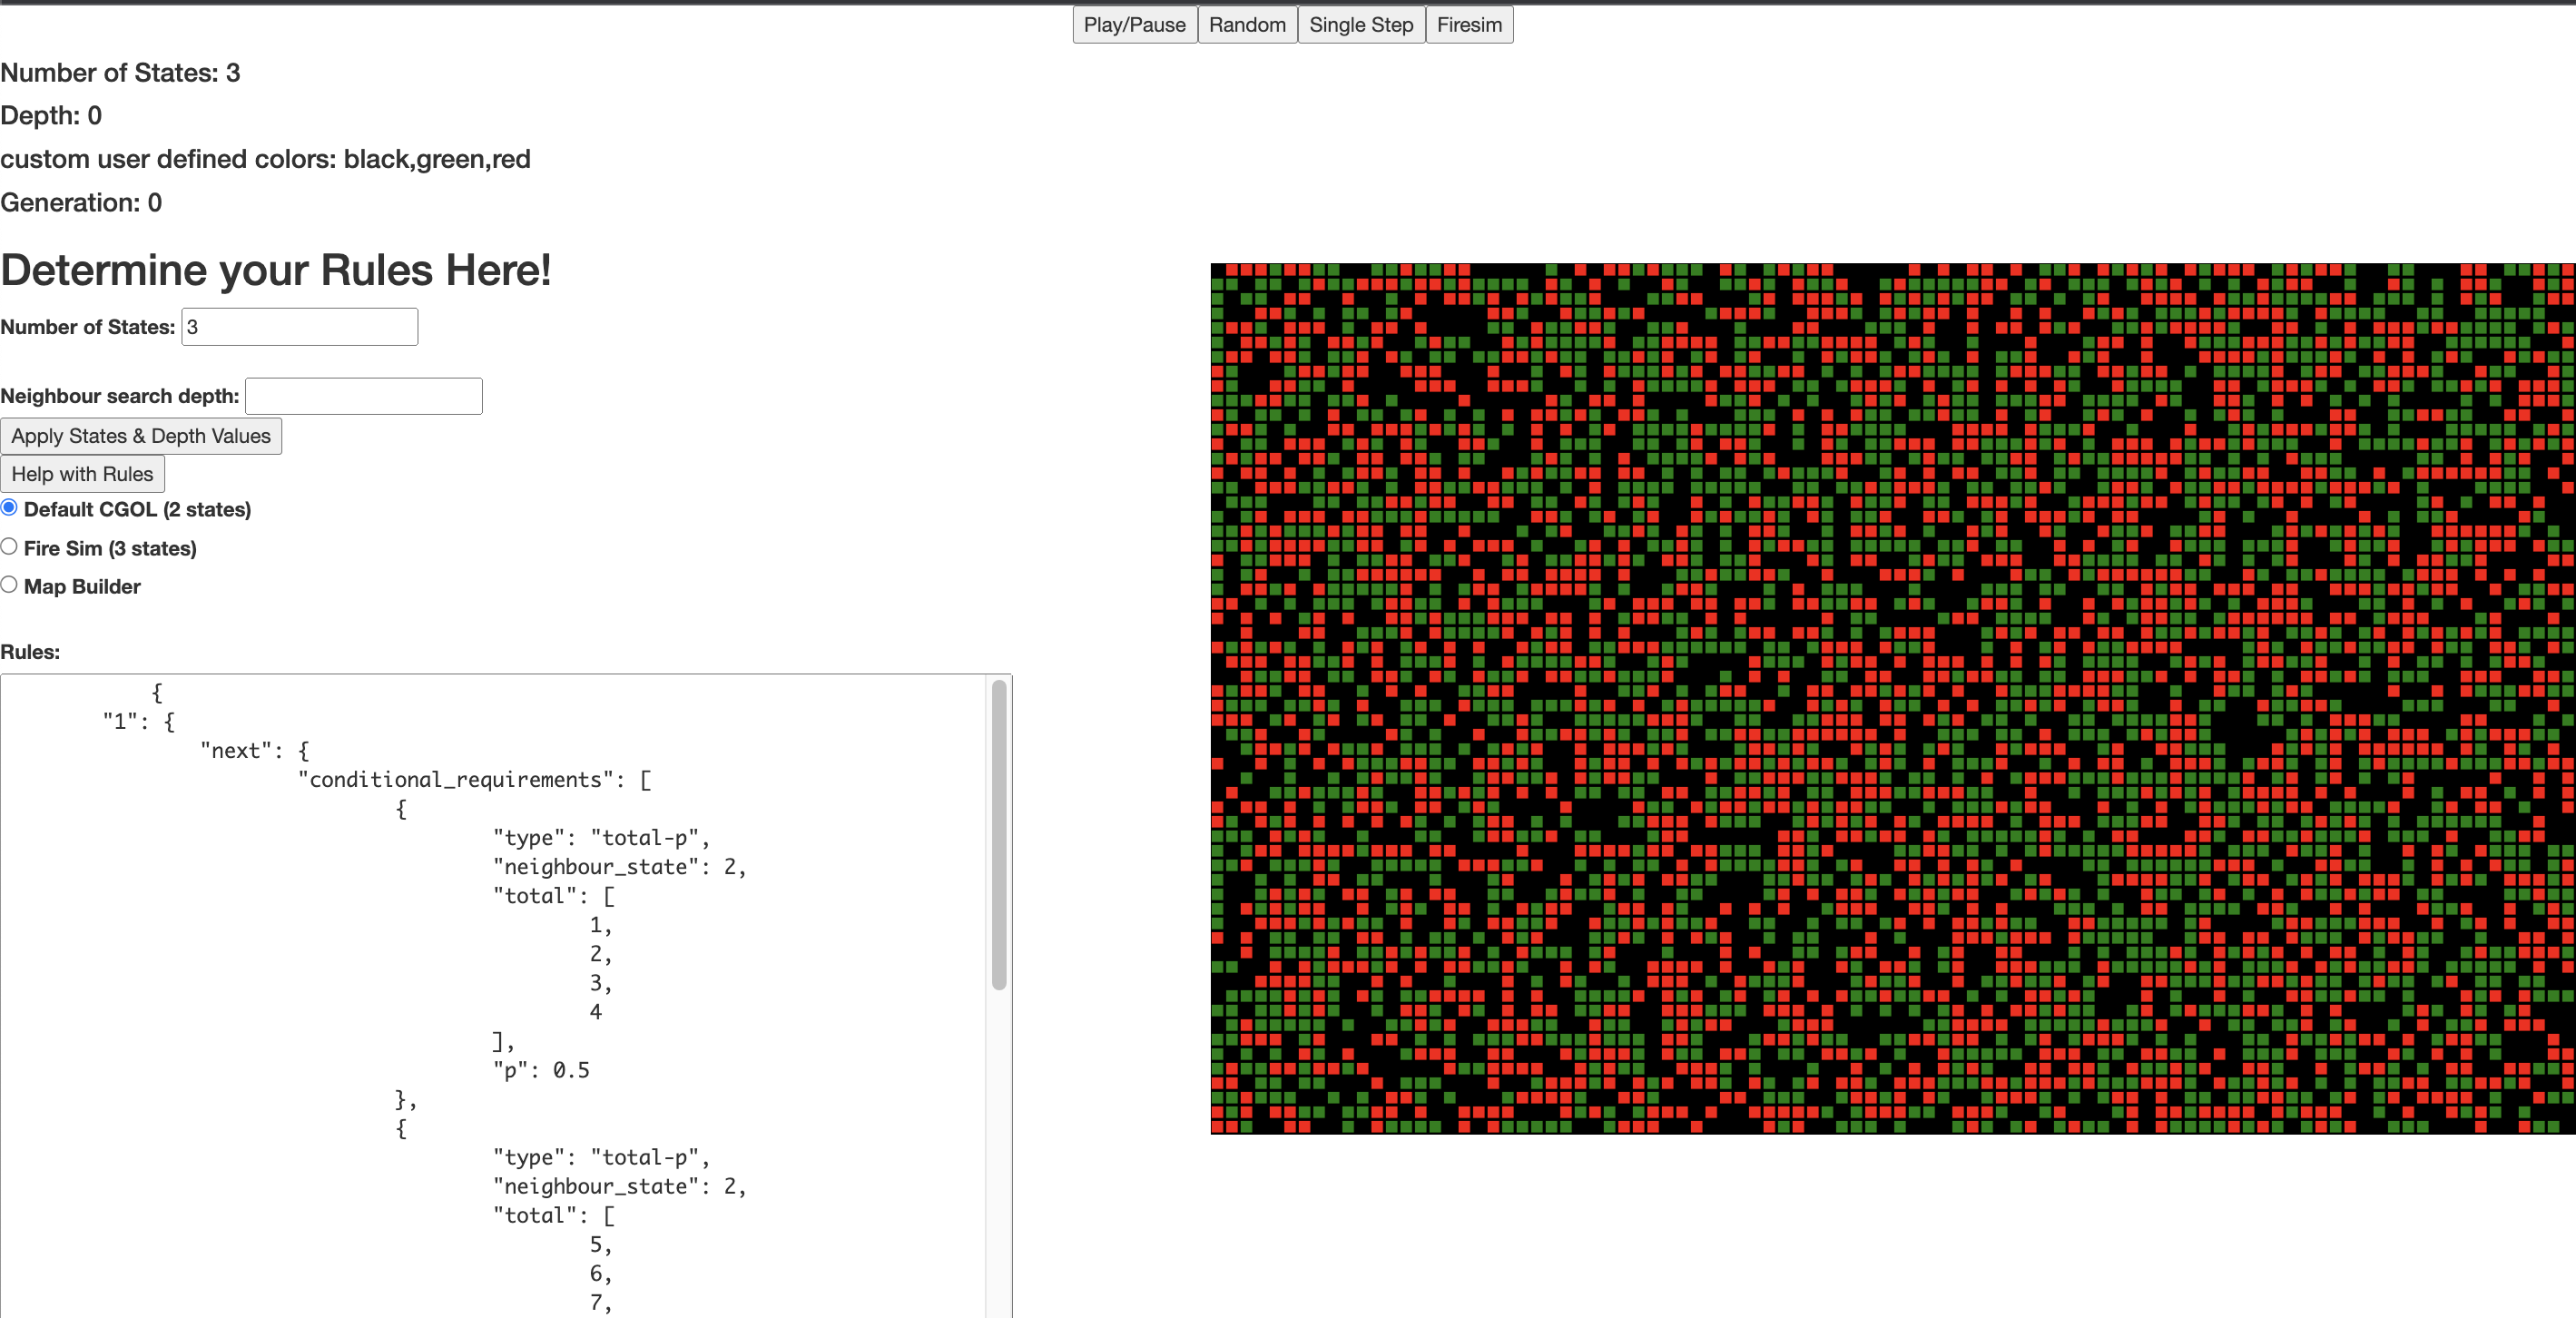
\includegraphics[scale=0.30]{gui_final.png}
\end{figure}
\\
In the end, a number of changes were added to the buttons section outlined from the early sketch above by the addition of states and color descriptions, and the number of elapsed generations. Additionally, two input fields, each for \textit{depth} and \textit{states} are presented. The buttons, on the other hand, have been moved to the center top of the page. 

\subsection{Dynamic Rules Components}
The dynamic rules components are a collection of functionalities that allow the input, output and preparation of user-defined rules for validation. In the GUI, this component will form the back and front end parts of the rules section. 
\\ \\
The editor is essentially a set of radio buttons, a customized HTML textarea component, and a 'submit' button to try and apply any user-defined rules.  The rule editor (textarea) element also serves the purpose of a 'display' of the currently adopted rules of the system. The radio buttons allow for instant changes to the editor content to any system default rules. How this works is that a new textarea of the same size is rendered, based on the changes made in the radio button, as the preset rules are changed. 
\\ \\
In the code, the dynamic rules component can be located in the \texttt{dynamic-rules-form.js} file in the \texttt{utils} folder. This component utilizes the functionality of the validator component (described in \ref{validator}), and passes the rules defined by the user to the function builder (described in \ref{f_builder}) when appropriate.

\subsection{Rules Format} \label{rules_format}
User-defined rules take the form of a JSON object (see section \ref{json_schema}) with a few objects contained by its mandatory keys. 
\\ \\
The use of a JSON format for the rules is due to its flexibility in defining nested JSON entities within its keys. Alternative formats were considered, e.g. XML, and so were different approaches (e.g. having the user write their own JavaScript functions). However, the JSON format is adopted as it's simpler and easily understandable for users due to the fact that users won't have to mark up every term \cite{haq2013comprehensive}.
\\ \\
Though the entire structure is validated against a JSON schema (see appendix \ref{json_schema}), the rules have two required objects and keys: \texttt{\$\_meta} and \texttt{default}. 
Their descriptions are described in the following:
\begin{itemize}
    \item \texttt{\$\_meta}: 
    The object holding this key contains two additional objects with the following keys: \texttt{num\_states} and \texttt{colors}
    \begin{itemize}
        \item \texttt{num\_states}: The \texttt{num\_states} key contains a single positive integer value that identifies the number of states the rules cover.
        \item \texttt{colors}: The \texttt{colors} object essentially outlines the colors associated to each state. Assume the above key \texttt{num\_states} contains Integer \textit{N}. The \texttt{colors} object should contain numeric keys from 0 to \textit{N-1} where each key contains string representing a color. These strings can be verbal color identifiers (e.g. red, blue), hexadecimal representations, RGB triples, or numbers between 0-255 (for grayscale colors)
    \end{itemize}
    \item \texttt{default}: The \texttt{default} object defines a state transition rule. The \texttt{default} object contains the key \texttt{next}, which in turn contains the following objects that satisfy a state transition rule:
    \begin{itemize}
        \item \texttt{conditional\_requirements}: The \texttt{conditional\_requirements} key contains a list of objects describing conditions to determine the next state. Each conditional requirement observes the neighbours of the cell, but does so in four different ways. The \texttt{type} key indicates the way they consider the roles of the neighbours. Depending on the value of \texttt{type}, the type of requirement calls for different parameters (keys) used to determine its satisfiability.
        Below are the accepted values for key \texttt{type}, how they observe neighbours, and their own required keys. 
        \\ \\
        The following table outlines the required additional arguments for each type of conditional requirements:
        \begin{table}[]
\begin{tabular}{|l|l|}
\hline
\multicolumn{1}{|c|}{\textbf{Type}} & \multicolumn{1}{c|}{\textbf{Additional Required Arguments}}                                                                                                                                   \\ \hline
"totalling"                         & \begin{tabular}[c]{@{}l@{}}neighbour\_state (int)\\ total (array{[}int{]})\end{tabular}                                                                                                       \\ \hline
"probability"                       & p (float)                                                                                                                                                                                     \\ \hline
"total-p"                           & \begin{tabular}[c]{@{}l@{}}neighbour\_state (int)\\ total (array{[}int{]})\\ p (float)\end{tabular}                                                                                           \\ \hline
"expression"                        & \begin{tabular}[c]{@{}l@{}}lhs (object: neighbour\_states (array(int)))\\ cmp (enum: {[}"\textless{}", "\textgreater{}", "="{]}) \\ rhs (object: neighbour\_states (array(int)))\end{tabular} \\ \hline
\end{tabular}
\caption{Table showing Required Arguments for Each Type of Conditional Requirements}
\end{table}
        \begin{enumerate}
            \item \texttt{totalling}: The \texttt{totalling} type of a cellular automata indicates that a cell looks for a certain state type in all its neighbours. If a cell has a certain number of neighbours in a specific state, then transition conditions are met. An example use case of these rules would be in CGOL. 
            \\
            Required keys:
            \begin{itemize}
                \item \texttt{neighbour\_state}: integer, indicating which state to look for in its neighbours
                \item \texttt{total}: list of integers, where if the total number of neighbours with state \texttt{neighbour\_state} are in the list, then state transition requirement is fulfilled. 
            \end{itemize}
            \item \texttt{probability}: \label{probability_condreq}
            The \texttt{probability} type requirement simply outputs \textit{True} or \textit{False} depending on the provided parameter \texttt{p} (for probability). \\
            Required keys:
            \begin{itemize}
                \item \texttt{p}: floating point number between 0 and 1.
            \end{itemize}
            \item \texttt{total-p}: The \texttt{total-p} type is a mixture of both the \texttt{totalling} and \texttt{probability} type. This means that if given a cell that has a certain number of neighbours in a certain state, it has a certain probability of transitioning to another state. An example use case of this state transition condition is of forest fire propagation \\
            Required keys:
            \begin{itemize}
                \item \texttt{p}: floating point number between 0 and 1.
                \item \texttt{neighbour\_state}: integer, indicating which state to look for in its neighbours
                \item \texttt{total}: list of integers, where if the total number of neighbours with state \texttt{neighbour\_state} are in the list, then has probability \texttt{p} of transitioning.
            \end{itemize}
            \item \texttt{expression}:
            The \texttt{expression} type of requirement is unique from the others categorical types as it looks for multiple states from its neighbours. \\
            Required keys:
            \begin{itemize}
                \item \texttt{lhs}: a list of ints indicating state types
                \item \texttt{cmp}: a comparator (i.e. \textless, \textgreater, etc.)
                \item \texttt{rhs}: a list of ints indicating state types
            \end{itemize}
            Essentially, this condition checks if neighbour's states defined in \texttt{lhs} are of a certain relation \texttt{cmp} compared to \texttt{rhs}
        \end{enumerate}
        \item \texttt{satisfied} and \texttt{else} keys: These two keys contain an integer outlining which state it should transition to, depending on the satisfaction of the described conditional requirements (preceding key). If any of the conditions in \texttt{conditional\_requirements} are met, then transition to state \texttt{satisfied}. Otherwise to \texttt{else}.
    \end{itemize}
\end{itemize}
More objects identified by numeric keys (associating to individual states) can be defined with the exact same properties of the \texttt{default} object, ultimately defining an outer totalistic cellular automata. 
\\ \\
The UML diagram of the rules format is shown below. Note that the following diagram's purpose is only to visualize the relationships between each fields:
\\
\begin{figure}[H]
    \caption{Rules Format in a UML Diagram}
    \centering
    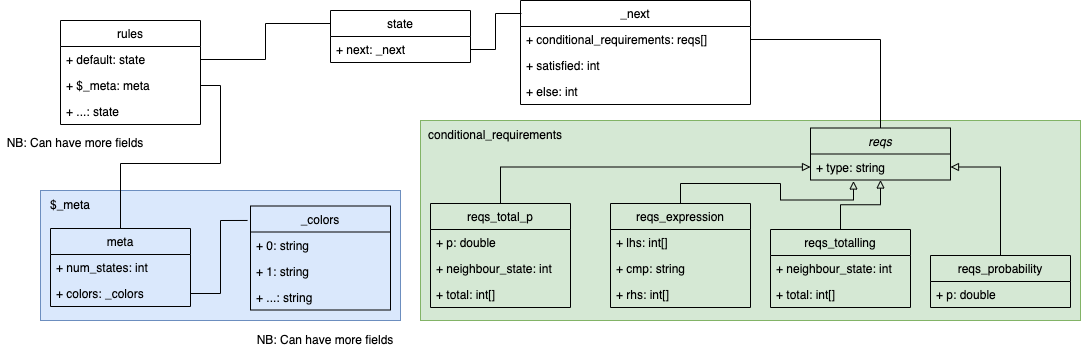
\includegraphics[scale=0.4]{uml_rules.png}
    \label{uml_rules}
\end{figure}

\noindent Overall, the reason of nesting the \texttt{conditional\_requirements}, \texttt{satisfied} and \texttt{else} keys in a \texttt{next} key after the state is mainly for code readability, particularly in the function builder, e.g. compare \texttt{json\_rules[0].satisfied} to \texttt{json\_rules[0].next.satisfied}. I argue the latter is more readable and verbose.

\newpage
\subsubsection{Examples of the Rules}
In order to grasp a better understanding of the rules, some examples are necessary. Their relationships are visualized in Figure \ref{uml_rules} above for reference. 
\\ \\
The general structure of the rules take the following form:
\\
\begin{center}
\begin{figure}[H]
\begin{verbatim}

                            {
                              $_meta: { ... },
                              default: { ... },      
                              0: { ... },
                              1: { ... },
                              ...
                            }
    
\end{verbatim}
\caption{General Structure of Rules}
\end{figure}
\end{center}
Note that the dots between the curly braces indicate a nested JSON object. The \texttt{\$\_meta} object only contains two key-value pairs. Below is an example of what the object may look like, and illustrates three valid ways of defining colors in the rules:
\begin{center}
\begin{figure}[H]
\begin{verbatim}
        
                            $_meta: {
                              num_states: 3,
                              colors: {
                                0: "red",
                                1: 255,
                                2: "#FF0000"
                              }
                            }
                
\end{verbatim}
\caption{Structure of \texttt{\$\_meta} object}
\end{figure}
\end{center}
As the previous section has stated, objects contained in the \texttt{default} key and any other numeric keys (0, 1, 2, etc.) contain the same structure. These objects are the \textbf{state transition rules}. In the following example, the \texttt{default} key contents will be shown:
\begin{center}
\begin{figure}[H]
\begin{verbatim}
        
                            default: {
                              next: {
                                conditional_requirements: [{ ... }],
                                satisfied: 1,
                                else: 0
                              }
                            }
                
\end{verbatim}
\caption{Structure of a basic state transition rule}
\end{figure}
\end{center}
The keys \texttt{satisfied} and \texttt{else} contain plain integers. The \texttt{conditional\_requirements} key contains a key of objects with the following formats:
\begin{center}
\begin{figure}[H]
\begin{verbatim}
        
                            conditional_requirements: [
                                {
                                  type: "totalling",
                                  neighbour_state: 1,
                                  total: [3],
                                }, 
                                {
                                  type: "probability",
                                  p: 1,
                                },
                                {
                                  type: "total-p",
                                  neighbour_state: 2,
                                  total: [1, 2, 3, 4],
                                  p: 0.8,
                                },
                                {
                                  type: "expression",
                                  lhs: {
                                    neighbour_states: [3, 4],
                                  },
                                  cmp: ">",
                                  rhs: {
                                    neighbour_states: [1, 2],
                                  },
                                }
                            ]
                
\end{verbatim}
\caption{Structure of conditional requirements list and different ways of specifying requirements}
\label{condreqslist_example}
\end{figure}
\end{center}
\noindent There are four ways of specifying a requirement for transition. And as shown in the Diagram in Figure \ref{uml_rules}, each variation of the requirements inherit the \texttt{type} parameter from its parent. For the above Figure \ref{condreqslist_example}, each requirement above can be translated to the following words in plain English, presented by the following table: 
\begin{table}[H]
\begin{tabular}{|l|l|}
\hline
\multicolumn{1}{|c|}{\textbf{Conditional Requirement}}                                                                                                                           & \multicolumn{1}{c|}{\textbf{Meaning}}                                                                      \\ \hline
\begin{tabular}[c]{@{}l@{}}\texttt{type: "totalling",}\\ \texttt{neighbour\_state: 1,}\\ \texttt{total: {[}3{]}}\end{tabular}                                                                              & There are a total of THREE neighbours with state ID 1                                                                        \\ \hline
\begin{tabular}[c]{@{}l@{}}\texttt{type: "probability",}\\ \texttt{p: 1}\end{tabular}                                                                                                             & There is a probability of 1                                                                                                  \\ \hline
\begin{tabular}[c]{@{}l@{}}\texttt{type: "total-p",}\\ \texttt{neighbour\_state: 2,}\\ \texttt{total: {[}1, 2, 3, 4{]},}\\ \texttt{p: 0.8}\end{tabular}                                                             & \begin{tabular}[c]{@{}l@{}}If there are 1, 2, 3, 4 neighbours with state ID 2, \\ there is a probability of 0.8\end{tabular} \\ \hline
\begin{tabular}[c]{@{}l@{}}\texttt{type: "expression",}\\ \texttt{lhs: \{}\\ \texttt{neighbour\_states: {[}3, 4{]},}\\ \},\\ \texttt{cmp: "\textgreater{}",}\\ \texttt{rhs: \{}\\ \texttt{neighbour\_states: {[}1, 2{]}} \\ \texttt{\}}\end{tabular} & If there are more of states 3 and 4 than 1 or 2                                                                              \\ \hline
\end{tabular}
\caption{Table of Interpretation from Rules to its meaning in English}
\label{rules_to_english_table}
\end{table}
\newpage
\subsection{Validator Component} \label{validator}
The Validator component is a standalone micro-component that compares the user-defined rules against the aforementioned JSON schema. Its functionality is called in the \\ \texttt{dynamic-rules-form.js} in validating the textarea's contents, in the form of the function \texttt{obeysJsonSchema()}. This component is an implementation of the TV4 library described in \ref{tv4}. 
\\ \\
The design choice of building the validator as the implementation of the TV4 library compared against a JSON schema is a practical choice done to save time. Developing an algorithm specific to this use case of iterating and testing the validity manually will require a great deal of time for research and implementation attempts. A general diagram on how the validator micro-component works is shown below:
\\
\begin{figure}[H]
    \caption{Validator Component Diagram}
    \centering
    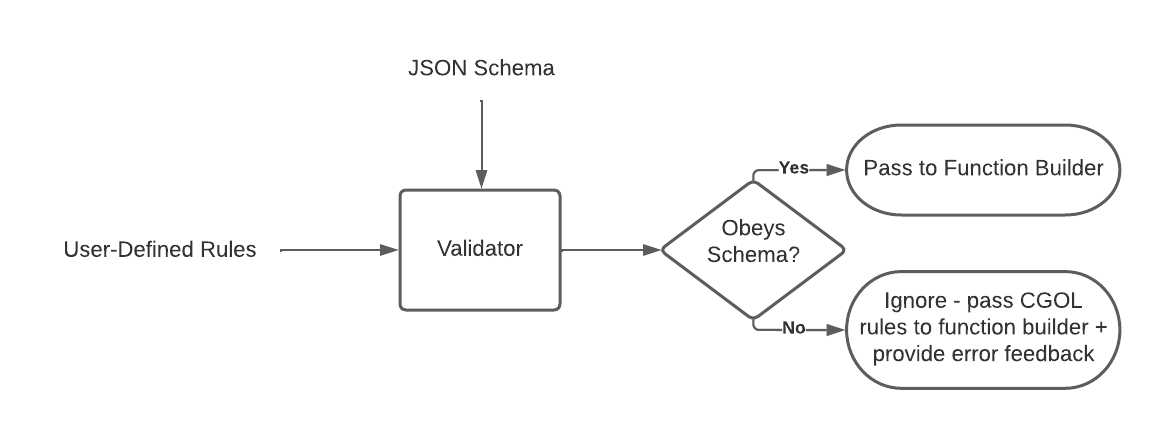
\includegraphics[scale=0.9]{validator_module.png}
\end{figure}
\noindent The validator attempts to determine the validity of rules passed to it in the system by parsing it (check to see if it's a valid JSON document), and the validity of it will be obtained by comparing against the provided JSON schema. Should the rules return invalid (or fail to parse), the validator will default to one of the system-default rules in the system, preventing the software to break.
\\ \\
The standalone \texttt{.js} file provided in the GitHub repository \ref{tv4} had a few integration problems such that the library was unable to use my supplied JSON schema \ref{json_schema} despite being able to use it online. That meant the simulator's validator had to use the Node Package variant of the library. 
\\ \\
The \textbf{Browserify} library was then used to compile the TV4 to yet another standalone \texttt{.js } file so it can provide support for browser applications \cite{browserify}.
\newpage

\subsection{Function Builder} \label{f_builder}
The function builder will accept values approved by the validator. This will either be one of the system's default rules, or the valid user-defined rules provided from the rule editor. CA rules have the capability of being defined by conditional statements (i.e. if-else statements). The pipeline of the function creator component will consist of parsing the given \texttt{conditional\_requirements} from the provided rules into if-statements, and then passed as an anonymous function to be used as the simulator's transition rules. 
\\ \\
The design of each the components making up the function builder component will now be described in the following subsections. This component and other micro-components contained can be found in the \texttt{function-builder.js} file in the \texttt{utils} folder. 
\\ \\
Overall, there are three major micro-components of the function builder: that is the condition builder, the if-statement builder, and the anonymous function builder. The architectural diagram for this module's running is provided as below:
\\
\begin{figure}[H]
    \caption{Function Builder Component and Micro Components}
    \centering
    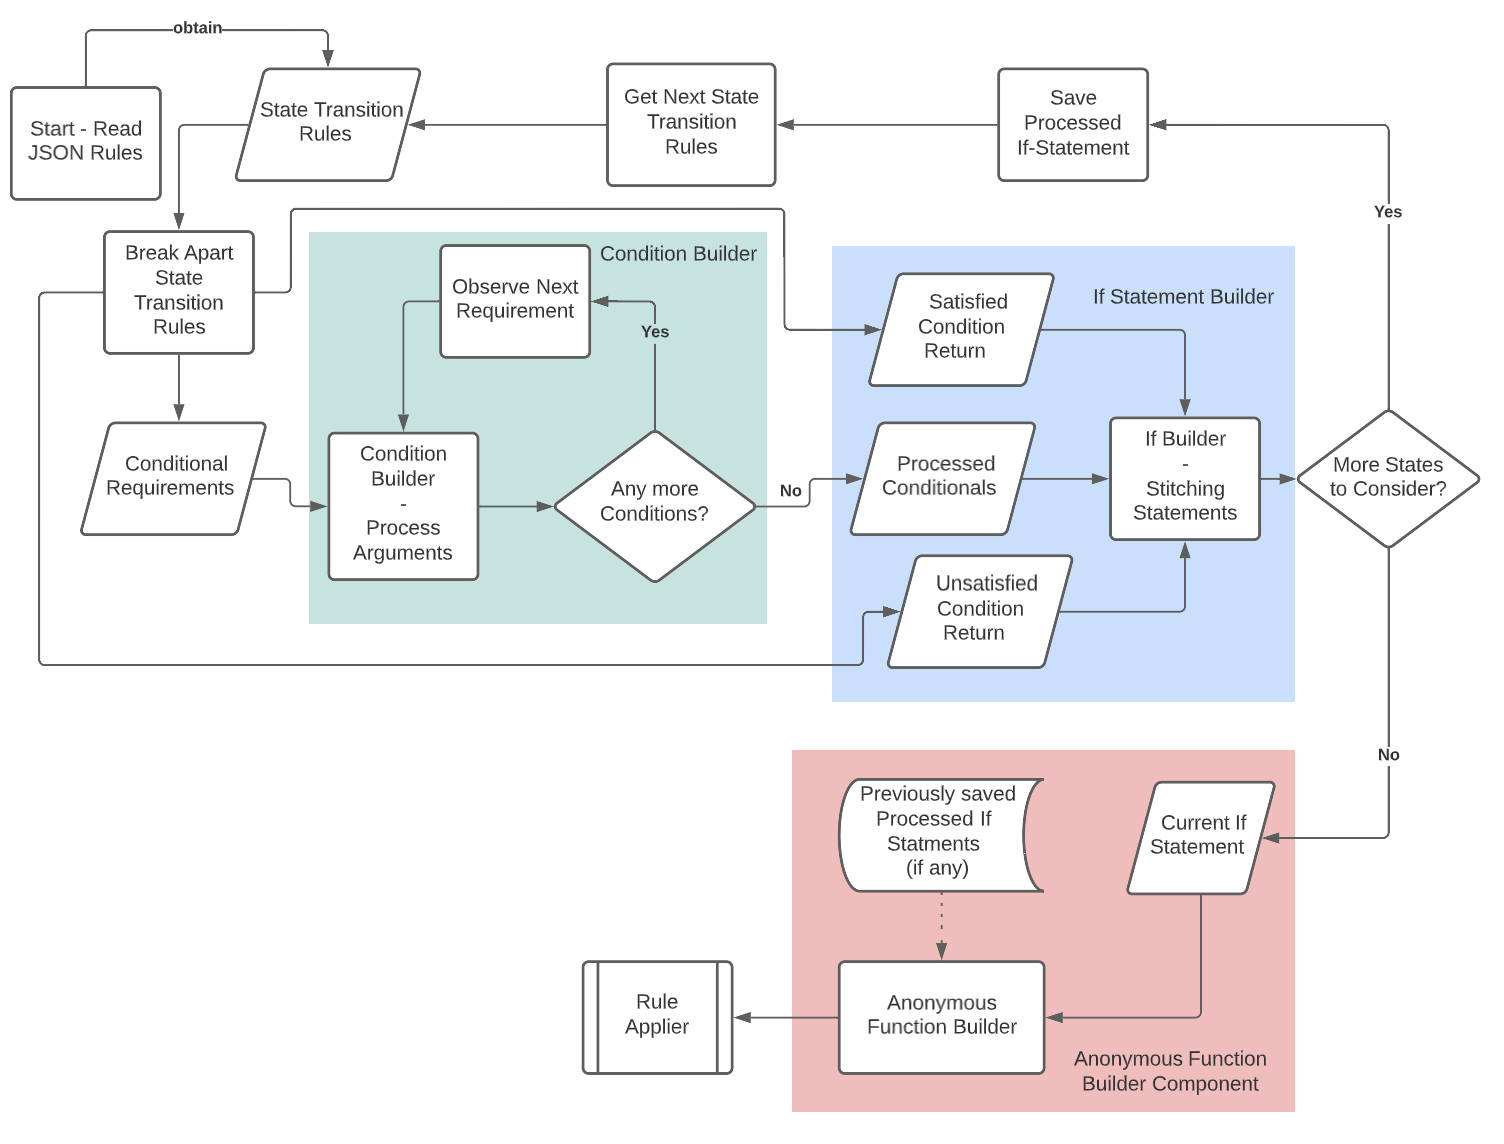
\includegraphics[scale=0.70]{functionbuilder_module.png}
\end{figure}
\subsubsection{Condition Builder}
I define conditions in this project as the values that are placed inside an if-statement. The condition builder is a micro-component within the function builder component that processes the inner most values of the rules from the format, i.e. the \texttt{conditional\_requirements} list. As described in section \ref{rules_format} on the rules format, the condition builder builds four types of conditions. 
\\ \\
Referring to Table \ref{rules_to_english_table}, the conditional requirements are translated into the following conditions in the following format:
\begin{table}[H]
\begin{tabular}{|l|l|}
\hline
\multicolumn{1}{|c|}{\textbf{Conditional Requirement}}                                                                                                                           & \multicolumn{1}{c|}{\textbf{Resulting Conditional}}                                                                      \\ \hline
\begin{tabular}[c]{@{}l@{}}\texttt{type: "totalling",}\\ \texttt{neighbour\_state: 1,}\\ \texttt{total: {[}3{]}}\end{tabular}                                                                              & \texttt{[3].includes[neighbours[1]]}                                                                        \\ \hline
\begin{tabular}[c]{@{}l@{}}\texttt{type: "probability",}\\ \texttt{p: 1}\end{tabular}                                                                                                             & \texttt{probability(1)}                                                                                               \\ \hline
\begin{tabular}[c]{@{}l@{}}\texttt{type: "total-p",}\\ \texttt{neighbour\_state: 2,}\\ \texttt{total: {[}1, 2, 3, 4{]},}\\ \texttt{p: 0.8}\end{tabular}                                                             & \begin{tabular}[c]{@{}l@{}} \texttt{(probability(0.8) \&\&} \\ \texttt{[1,2,3,4].includes(neighbours[2])} \end{tabular} \\ \hline
\begin{tabular}[c]{@{}l@{}}\texttt{type: "expression",}\\ \texttt{lhs: \{}\\ \texttt{neighbour\_states: {[}3, 4{]},}\\ \},\\ \texttt{cmp: "\textgreater{}",}\\ \texttt{rhs: \{}\\ \texttt{neighbour\_states: {[}1, 2{]}} \\ \texttt{\}}\end{tabular} & \texttt{neigh[3] + neigh[4] \textgreater{} neigh[1] + neigh[2]}                                                                    \\ \hline
\end{tabular}
\caption{Translation Table from Rules to JS Conditions Implementation}
\label{rules_to_english_table}
\end{table}
\noindent Important to note that \texttt{neigh} is the same as \texttt{neighbours} and are dictionaries. They are defined in Section \ref{ncrc} and are allocated every cell. In essence, \texttt{neighbours[1]} holds the amount of type \texttt{1} neighbours the cell in test has.
\\ \\
When there are multiple conditional requirements provided in the list, then the conditionals are connected via an \texttt{OR} connection. There was no specific reason in choosing to connect the conditionals with an \texttt{OR} instead of \texttt{AND}, apart from the fact that configuring the connectives could be a feature to be added another day.

\subsubsection{Probability Calculator (Micro Component)} \label{prob_calc_fbuilder}
The probability calculator micro component complements the functionality of the condition builder. Its purpose is defined above in number \ref{probability_condreq} of the \texttt{type} key value of the \\ \texttt{conditional\_requirement} object. Its evaluation, however, is called in the Actuator component. That being said, it is not shown in the diagram. Its overall usage is described in the \ref{actuator} subsection below.

\subsubsection{If Builder}
The If Builder is a straightforward micro-component that accepts values (conditions) passed from the condition builders. It takes two integer arguments (\texttt{satisfied\_rtn} and \texttt{otherwise}) for the states to transition to, and a string argument \texttt{conditions}. This micro-component simply returns a literal string value of the built if statement.

\subsubsection{Anonymous Function Generator}
Once the rules are read and the appropriate micro-components are utilized, the final part of the function builder relies on a JS anonymous function builder. The anonymous functions are then passed to the actuator, where the rules are ultimately applied in the simulator.

\subsection{Actuator} \label{actuator}
The actuator will function as the simulator's back-end. Two major functionalities of the actuator is counting the Moore Neighbours of each cell in the CA and applying the rules supplied by the function builder. These functionalities are triggered by the buttons. Additionally, the actuator is the first component that is called to action in the system as it renders the entire page as the \texttt{setup()} function is executed in the \texttt{sketch.js} file. The \texttt{setup()} function operates quite trivially as it only assigns the default starting variables, and it therefore won't be discussed here. 
\subsubsection{Initializer} \label{initializer}
The initializer is a micro-component for the actuator. It is the first part of the actuator that is called when a user accesses the tool, or make changes to the rules and system. More importantly, the initializer renders the front end. This component is therefore both a back-end and a front-end component. In essence, the initializer determines the following variables:
\begin{itemize}
    \item \textbf{Number of States}: This variable is supplied to a variety of components, i.e. the color allocator micro component (see \ref{color_allocator})
    \item \textbf{Active Rules}: The active rules are the transition rules for the simulator, after the approval from the validator component (see \ref{validator}) and processed by the function builder (see \ref{f_builder}). 
    \item \textbf{2D Array Dimensions}: These dimensions (rows and columns) are determined in this setup. These values are passed on to the respective 2D Array Creator (see subsection below).
\end{itemize}

\subsubsection{Two-Dimensional Array Creator (Micro Component)} \label{2darr_creator}
As the heading suggests, the actuator contains a two-dimensional array creator. This functionality is used by the initializer (see above) and by the Rule Applier micro component within this component (see \ref{ncrc}). Two-dimensional arrays are used as the CA simulator two-dimensional grid, thus emphasizing its importance. 
\\ \\
Rows and Columns of this two-dimensional array are calculated by dividing the width and height of the user's screen with the resolution.
\newpage
\subsubsection{Color Allocator (Micro Component)} \label{color_allocator}
The color allocator is a micro component within the actuator that focuses on color allocation for each state. In essence, it returns an Array whose indexes correspond to the state number, and the contents contained at the index is the state's color. For example, consider a five-state CA with states labelled from 0-4:
\begin{figure}[H]
    \caption{State Number Corresponding to Color}
    \centering
    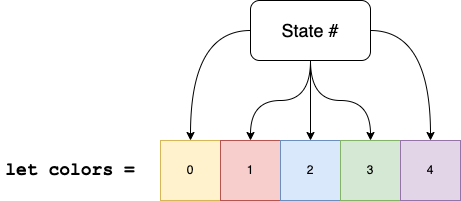
\includegraphics[scale=0.50]{aoc.png}
\end{figure}
\noindent The color of State \# 0 is therefore contained in \texttt{colors[0]} (yellow), State \# 1 in \texttt{colors[1]}, and so on. The color of state \# k is contained in \texttt{colors[k]}.
\\ \\
The allocator firstly checks whether the \texttt{colors} key exists in the \texttt{\$\_meta} object and if the number of states are equal to the number of keys contained in \texttt{colors}, and they values contained in the keys are of valid color representations. Otherwise, random colors are allocated to the states. The flowchart of this micro-component can be seen below:
\\
\begin{figure}[H]
    \caption{Color Allocator Flowchart}
    \centering
    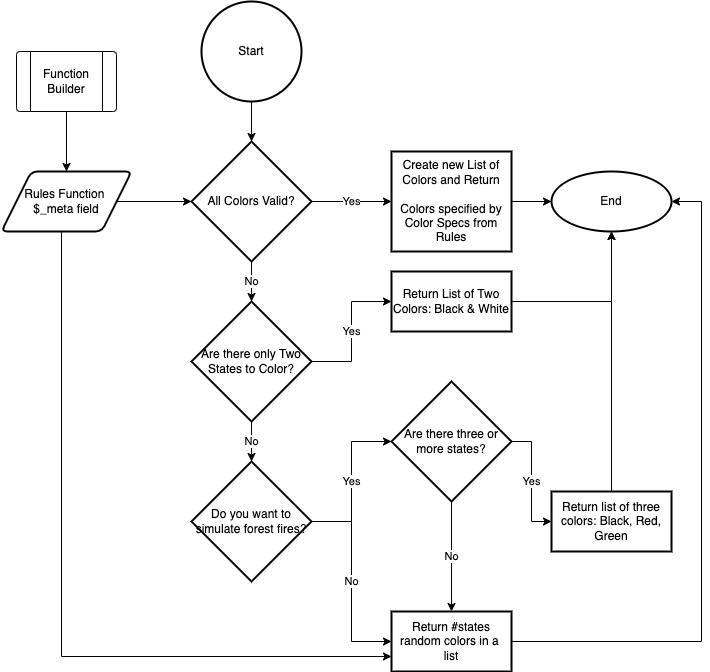
\includegraphics[scale=0.45]{flowchart_coloralloc.drawio.png}
\end{figure}
\newpage
\subsubsection{Actuator Buttons}
The buttons (seen in the top part of figure \ref{fig:final_gui}) serve as the inputs (operating similarly to remote) to the actuator. Though the buttons are essentially rendered as part of the GUI, its main functionality is defined in the actuator class. The following buttons are provided, and their actions:
\begin{itemize}
    \item Play/Pause: 
    There is a \texttt{pause} variable of type \texttt{boolean} in the system that drives whether the simulator should execute or not. While \texttt{pause} is initially set to \textit{True}, this button negates the value of \texttt{pause}, where there is another function \texttt{draw()} essentially runs the simulator. 
    \item Single Step: 
    The single step button operates the same way as the play/pause button, but what this button does in a single run is explicitly declare \texttt{pause} to \textit{True}, calls the \texttt{draw()} function, and then resets \texttt{pause} to \textit{False}
    \item Randomize:
    The randomize button essentially creates a new two-dimensional array according to the number of states and associated number of If colors are not provided to each state from the \texttt{\$\_meta} tag, then they are randomly allocated by the color allocation micro-component above in section \ref{color_allocator}.
\end{itemize}
The flowcharts for the buttons are shown below:
\\
\begin{figure}[H]
    \caption{Button Actions Flowchart}
    \centering
    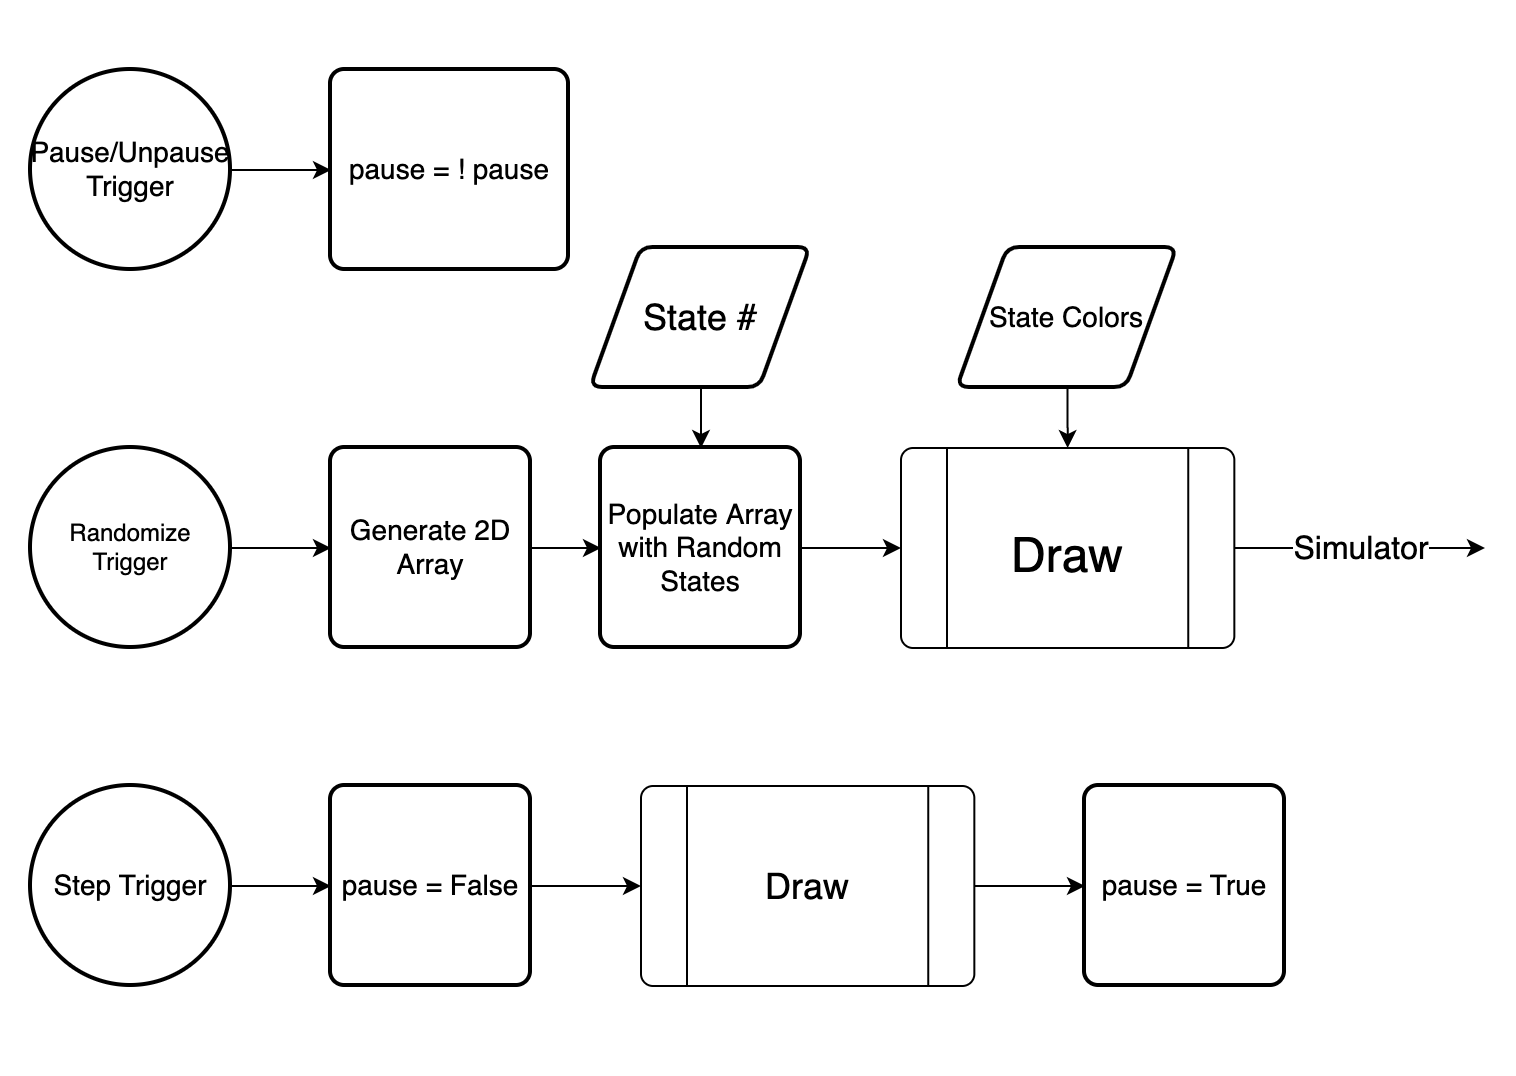
\includegraphics[scale=0.50]{buttonactions_module.png}
\end{figure}

\newpage
\subsubsection{Neighbour Counter \& Rule Applier} \label{ncrc}
CAs commonly consider the neighbour numbers and states before deciding what to do next. That being said, neighbour numbers and their states are typically calculated in one single function, that is when the rules are applied. However, integrating both functionalities into a single micro-component introduces a higher level of cognitive complexity in the algorithms, making it potentially harder to manage, and maybe even add features.
\\ \\
For that reason, these micro-components are separately defined (in different functions) for modularity. However, in the running process of the rule applier micro-component, it calls the function of the neighbour counter. Following is the flowchart of the Rule Applier:
\\
\begin{figure}[h]
    \caption{Rule Applier Flowchart}
    \centering
    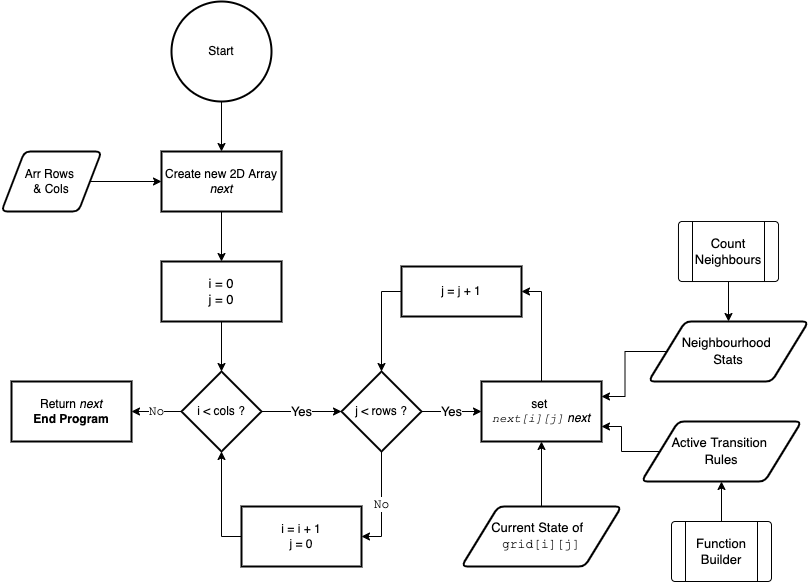
\includegraphics[scale=0.50]{ruleapplier.drawio.png}
\end{figure}
\\
The rule applier essentially creates a new two dimensional array of cells with the same dimensions as the current grid, iterates each cell from top left to bottom right by using a nested for-loop, assigning new states to the cells at the new array (with input from neighbour count and cell's current state). 
\newpage
\noindent The neighbour counter operates as specified by the following chart:
\begin{figure}[H]
    \caption{Neighbour Counter Flowchart}
    \centering
    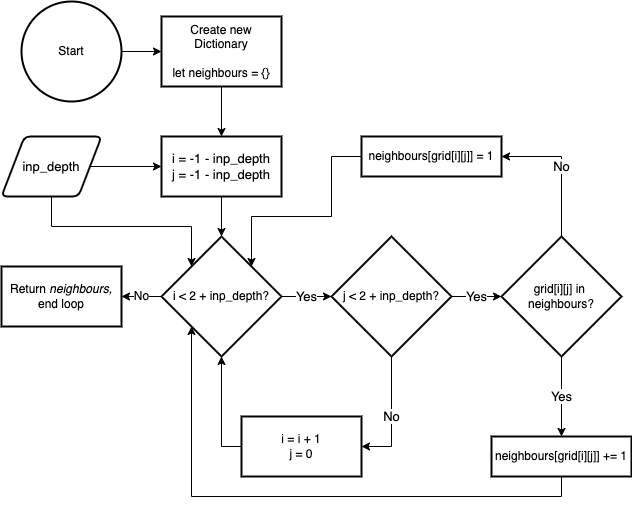
\includegraphics[scale=0.50]{flowchart_neighbourcounter.png}
\end{figure}

\noindent The design choice of implementing an infinite two-dimensional grid (instead of a finite grid in the provided frame) was made due to the fact that CAs are typically based on an infinite grid, particularly CGOL \cite{kier2005modeling}. The way this was implemented is reflected in the rule applier code, where the cells wrap around each other (e.g. bottom right cell's neighbour includes top left cell, and vice versa).
\newpage
\subsection{Sketcher}
The sketcher (or simulator) visualizes the current CA grid and its colors. This component has mostly stayed the same in the context of its GUI appearance, and is purely front end. It accepts two dimensional arrays containing the new state of the CA. This component utilizes the P5JS library, described in \ref{p5js}. A small part of the sketching process occurs in the highlighted area in the flowchart below:
\\
\begin{figure}[H]
    \caption{Flowchart of Sketcher}
    \centering
    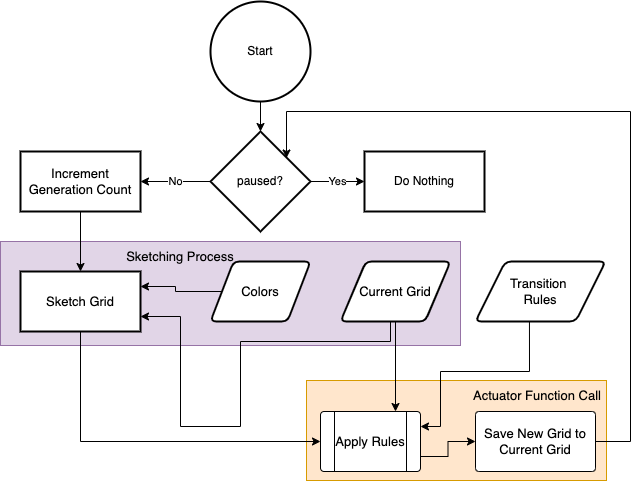
\includegraphics[scale=0.50]{flowchart_sketcher.png}
\end{figure}
\noindent The \texttt{sketch()} function attempts to visualize the CAs in the simulator. Additionally, this module calls the functionality of the actuator (indicated as well in the flowchart) to keep its process running.

\subsection{Help Page}
Finally, there is a basic help page that is essentially a static \texttt{.html} page. It describes the basics of CAs. Additionally, this page outlines a basic tutorial on how to use the tool, and more importantly learn the proper syntax of the rules to input to the system through the editor. As this component is a simple HTML page, no component diagram is specified, nor will this be represented in the general architectural diagram. 
\\ \\
The help page can be accessed through a button above the rules editor.
\newpage
\section{Dependency Graph}
This graph shows the dependencies needed by each of the written components in order to properly function. Arrows from component \textbf{A} pointing towards another component \textbf{B} signify that "component \textbf{A} depends on component \textbf{B}". Additionally, the external libraries are highlighted in the diagram.
\\
\begin{figure}[h]
    \caption{Dependency Diagram}
    \centering
    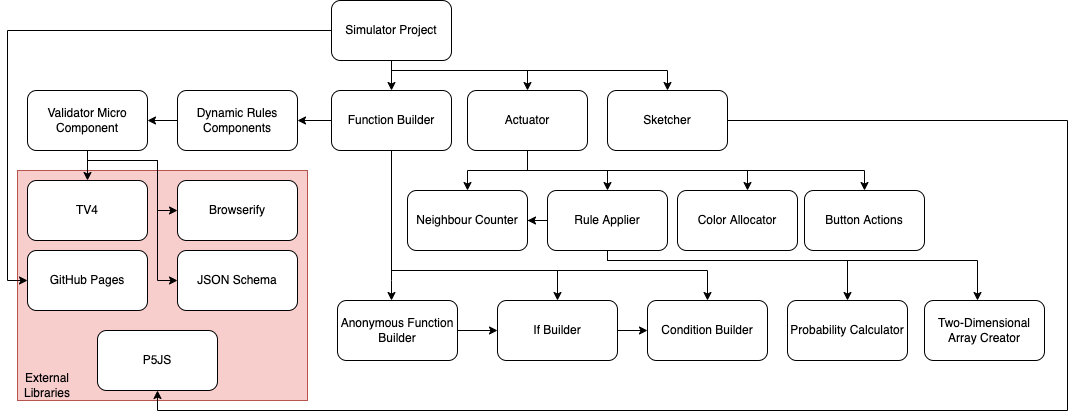
\includegraphics[scale=0.45]{dependency_diagram2.png}
\end{figure}
\\
Note that some component names were not listed such as the GUI (see \ref{gui_component}) and the Initializer (see \ref{initializer}) as their functionalities are purely front end. Inherently, they depend on each and every one of the components and form as part of the simulator project itself. 
\chapter{Testing \& Evaluation}

A known limitation of the system is that there is no user-friendly way of defining the dimensions of the CA simulator. That being said, to test the rules' accuracies and how well the simulation scales, some changes need to be made to the code base at the lower level. 
\\ \\
The scalability of the simulator is tested as the simulator size is dependent on the size of the computer screen. No performance enhancements will be made, as only the display size will be changed. 
\section{Simulation Scaling Test}
Before going to the details on the procedure of this test, it is important to understand how the program determines the dimensions of the two-dimensional array for the simulator. This is discussed in \ref{2darr_creator}.
We measure how well the simulation scales by measuring the amount of time taken between each generation's transition, i.e. how long it takes for the simulator to apply the transition rules to all the cells, and the average time taken to do so. The average time taken to transition between ten generations is the dependent variable. The independent variable will be a coefficient introduced to the resolution, as the size of the simulator is determined in the \texttt{setup()} function where the rows and column count are divided by the resolution. Only the code from the \texttt{sketch.js} file are changed to support logging. The following changes are introduced to the system to evaluate its scalability:
\begin{enumerate}
    \item A new Array \texttt{times\_10} will be made to store the times taken for transition between 10 generations.
    \item A new floating point number, \texttt{coeff} to be multiplied to the resolution in the \texttt{setup} function.
    \item The \texttt{draw()} function will automatically stop after ten iterations, then log the times taken. 
\end{enumerate}
The rules operated in this test will be the CGOL and Forest Fire Simulator Rules.
\newpage
\noindent It is important to note that the number of rows and columns for the grid are directly proportional to the resolution coefficient, as shown in the table below and the graph that follows:
\begin{table}[H]
\begin{tabular}{|c|c|c|}
\hline
\begin{tabular}[c]{@{}c@{}}Resolution \\ Coefficient\end{tabular} & Rows & Cols \\ \hline
1                                                                 & 60   & 96   \\ \hline
1.5                                                               & 90   & 144  \\ \hline
2                                                                 & 120  & 192  \\ \hline
2.5                                                               & 150  & 240  \\ \hline
3                                                                 & 180  & 288  \\ \hline
3.5                                                               & 210  & 336  \\ \hline
4                                                                 & 240  & 384  \\ \hline
4.5                                                               & 270  & 432  \\ \hline
\end{tabular}
\caption{Table of Resolution Coefficient to Rows and Columns}
\end{table}
\begin{figure}[H]
    \caption{Graph showing of Resolution Coefficient vs. no. of Rows and Columns}
    \centering
    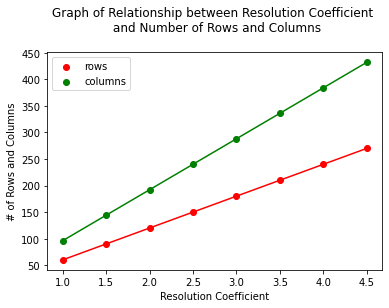
\includegraphics[scale=0.70]{linear_rows_cols.png}
\end{figure}
\noindent That being said, this section will observe the relationship between the coefficient (inherently the number of rows and columns) and the time it takes to apply the transition rules:
\begin{center}
\begin{table}[H]
\begin{tabular}{|c|cccccccccc|c|}
\hline
\begin{tabular}[c]{@{}c@{}}Resolution \\ Coefficient\end{tabular} & \multicolumn{10}{c|}{Generation Transition Times (ms)} & Average (ms) \\ \hline
1                                                                 & \multicolumn{1}{c|}{61}   & \multicolumn{1}{c|}{40}   & \multicolumn{1}{c|}{39}   & \multicolumn{1}{c|}{39}   & \multicolumn{1}{c|}{39}   & \multicolumn{1}{c|}{30}   & \multicolumn{1}{c|}{31}   & \multicolumn{1}{c|}{31}   & \multicolumn{1}{c|}{31}   & 32   & 37.3         \\ \hline
1.5                                                               & \multicolumn{1}{c|}{105}  & \multicolumn{1}{c|}{116}  & \multicolumn{1}{c|}{109}  & \multicolumn{1}{c|}{92}   & \multicolumn{1}{c|}{90}   & \multicolumn{1}{c|}{91}   & \multicolumn{1}{c|}{92}   & \multicolumn{1}{c|}{95}   & \multicolumn{1}{c|}{95}   & 95   & 98           \\ \hline
2                                                                 & \multicolumn{1}{c|}{548}  & \multicolumn{1}{c|}{564}  & \multicolumn{1}{c|}{559}  & \multicolumn{1}{c|}{498}  & \multicolumn{1}{c|}{508}  & \multicolumn{1}{c|}{506}  & \multicolumn{1}{c|}{507}  & \multicolumn{1}{c|}{509}  & \multicolumn{1}{c|}{465}  & 493  & 517.7        \\ \hline
2.5                                                               & \multicolumn{1}{c|}{645}  & \multicolumn{1}{c|}{609}  & \multicolumn{1}{c|}{626}  & \multicolumn{1}{c|}{552}  & \multicolumn{1}{c|}{595}  & \multicolumn{1}{c|}{586}  & \multicolumn{1}{c|}{623}  & \multicolumn{1}{c|}{552}  & \multicolumn{1}{c|}{590}  & 561  & 593.9        \\ \hline
3                                                                 & \multicolumn{1}{c|}{1434} & \multicolumn{1}{c|}{1307} & \multicolumn{1}{c|}{1254} & \multicolumn{1}{c|}{1209} & \multicolumn{1}{c|}{1213} & \multicolumn{1}{c|}{1156} & \multicolumn{1}{c|}{1169} & \multicolumn{1}{c|}{1174} & \multicolumn{1}{c|}{1180} & 1146 & 1224.2       \\ \hline
3.5                                                               & \multicolumn{1}{c|}{1876} & \multicolumn{1}{c|}{1759} & \multicolumn{1}{c|}{1790} & \multicolumn{1}{c|}{1923} & \multicolumn{1}{c|}{1822} & \multicolumn{1}{c|}{1748} & \multicolumn{1}{c|}{1703} & \multicolumn{1}{c|}{1786} & \multicolumn{1}{c|}{1686} & 1663 & 1775.6       \\ \hline
4                                                                 & \multicolumn{1}{c|}{2345} & \multicolumn{1}{c|}{1802} & \multicolumn{1}{c|}{1855} & \multicolumn{1}{c|}{1891} & \multicolumn{1}{c|}{1810} & \multicolumn{1}{c|}{1794} & \multicolumn{1}{c|}{1772} & \multicolumn{1}{c|}{1786} & \multicolumn{1}{c|}{1820} & 1954 & 1882.9       \\ \hline
4.5                                                               & \multicolumn{1}{c|}{3070} & \multicolumn{1}{c|}{2946} & \multicolumn{1}{c|}{3059} & \multicolumn{1}{c|}{2835} & \multicolumn{1}{c|}{2805} & \multicolumn{1}{c|}{2738} & \multicolumn{1}{c|}{2792} & \multicolumn{1}{c|}{2824} & \multicolumn{1}{c|}{2735} & 2644 & 2844.8       \\ \hline
\end{tabular}
\caption{Table of Resolution Coefficient and Generation Transition Times for CGOL Rules in ms}
\end{table}
\end{center}
\noindent From the table above, it can be seen that there is a positive correlation between the resolution coefficient and the average time taken for the transition to occur to the entirety of the CA grid. The same experiment can be done for the forest fire simulator rules. The results are provided in the table below:
\begin{table}[H]
\begin{tabular}{|c|cccccccccc|c|}
\hline
\begin{tabular}[c]{@{}c@{}}Resolution \\ Coefficient\end{tabular} & \multicolumn{10}{c|}{Generation Transition Times (ms)}                                                                                                                                                                                                           & Average (ms) \\ \hline
1                                                                 & \multicolumn{1}{c|}{45}   & \multicolumn{1}{c|}{22}   & \multicolumn{1}{c|}{23}   & \multicolumn{1}{c|}{26}   & \multicolumn{1}{c|}{27}   & \multicolumn{1}{c|}{28}   & \multicolumn{1}{c|}{24}   & \multicolumn{1}{c|}{23}   & \multicolumn{1}{c|}{40}   & 24   & 28.2         \\ \hline
1.5                                                               & \multicolumn{1}{c|}{93}   & \multicolumn{1}{c|}{98}   & \multicolumn{1}{c|}{76}   & \multicolumn{1}{c|}{81}   & \multicolumn{1}{c|}{80}   & \multicolumn{1}{c|}{72}   & \multicolumn{1}{c|}{80}   & \multicolumn{1}{c|}{92}   & \multicolumn{1}{c|}{76}   & 82   & 83.0         \\ \hline
2                                                                 & \multicolumn{1}{c|}{524}  & \multicolumn{1}{c|}{466}  & \multicolumn{1}{c|}{564}  & \multicolumn{1}{c|}{510}  & \multicolumn{1}{c|}{453}  & \multicolumn{1}{c|}{508}  & \multicolumn{1}{c|}{495}  & \multicolumn{1}{c|}{464}  & \multicolumn{1}{c|}{446}  & 478  & 490.8        \\ \hline
2.5                                                               & \multicolumn{1}{c|}{592}  & \multicolumn{1}{c|}{613}  & \multicolumn{1}{c|}{523}  & \multicolumn{1}{c|}{559}  & \multicolumn{1}{c|}{551}  & \multicolumn{1}{c|}{588}  & \multicolumn{1}{c|}{547}  & \multicolumn{1}{c|}{545}  & \multicolumn{1}{c|}{592}  & 566  & 567.6        \\ \hline
3                                                                 & \multicolumn{1}{c|}{1250} & \multicolumn{1}{c|}{1185} & \multicolumn{1}{c|}{1266} & \multicolumn{1}{c|}{1149} & \multicolumn{1}{c|}{1158} & \multicolumn{1}{c|}{1159} & \multicolumn{1}{c|}{1117} & \multicolumn{1}{c|}{1134} & \multicolumn{1}{c|}{1108} & 1084 & 1161.0       \\ \hline
3.5                                                               & \multicolumn{1}{c|}{1718} & \multicolumn{1}{c|}{1728} & \multicolumn{1}{c|}{1795} & \multicolumn{1}{c|}{1724} & \multicolumn{1}{c|}{1709} & \multicolumn{1}{c|}{1640} & \multicolumn{1}{c|}{1647} & \multicolumn{1}{c|}{1586} & \multicolumn{1}{c|}{1678} & 1591 & 1681.6       \\ \hline
4                                                                 & \multicolumn{1}{c|}{2029} & \multicolumn{1}{c|}{2188} & \multicolumn{1}{c|}{2294} & \multicolumn{1}{c|}{1850} & \multicolumn{1}{c|}{1901} & \multicolumn{1}{c|}{1799} & \multicolumn{1}{c|}{1896} & \multicolumn{1}{c|}{1886} & \multicolumn{1}{c|}{1800} & 1881 & 1952.4       \\ \hline
4.5                                                               & \multicolumn{1}{c|}{2551} & \multicolumn{1}{c|}{2658} & \multicolumn{1}{c|}{2552} & \multicolumn{1}{c|}{2547} & \multicolumn{1}{c|}{2509} & \multicolumn{1}{c|}{2511} & \multicolumn{1}{c|}{2520} & \multicolumn{1}{c|}{2545} & \multicolumn{1}{c|}{2575} & 2748 & 2571.6       \\ \hline
\end{tabular}
\caption{Table of Resolution Coefficient and Generation Transition Times for Forest Fire Simulator Rules in ms}
\end{table}
\noindent The curve below visualizes the relationship between the resolution coefficient and the average transition time from one generation to another. 
\begin{figure}[H]
    \caption{Graph showing of Resolution Coefficient vs. Avg. Transition Times}
    \centering
    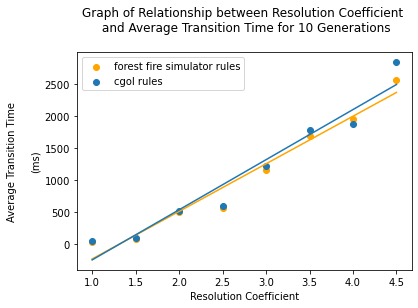
\includegraphics[scale=0.70]{plot_res_ttime.png}
\end{figure}
\noindent Based on the straight line and minimal signs of deviation, there is evidently a direct proportional relationship between the resolution coefficient and the average transition times. This is because the growth in number of rows and columns is directly proportional to the growth of the resolution coefficient. 

\newpage
\section{User Acceptance Testing}
In order to obtain feedback from users about this system's perceived usefulness, a qualitative interview was conducted. Two one-on-one interviews were conducted at different sittings. Both interview participants were computer science students at the University of Manchester. Each participant has also indicated familiarity with JSON and CAs (only CGOL). 
\\ \\
No personally identifiable data is collected during the interview. Both participants have indicated their consent in participating by signing a form, and are aware that participation is entirely voluntary and could withdraw from the interview at any point. 
\subsection{Setup and Methodology}
A document was created to act as a guide for the interviewees. This document was to be shown side-by-side the software in hand (see Appendix \ref{appendix:questionnaire}). Additionally, the Think Aloud method was adopted throughout the interview process. This means that the participants continuously spoke aloud any words that appear in their mind as they complete the tasks, and even up until concluding the interview \cite{charters2003thinkaloud}. I as the researcher was present beside the participant(s) to observe each of their thought processes, take notes, and provide support if required. 
\\ \\
Before conducting the interviews, one line of the code was changed. This change resulted in the radio button that populated the rules editor with the Map Generation CA (bottom left) to be hidden. This will prevent the participant in enabling the Map Generation CA rules, as the interview will involve the process of replicating the aforementioned rules (final part of Appendix \ref{appendix:questionnaire}). The Appendix also serves as the questions asked throughout the interview.

\subsection{Understanding the User Interface}
This part of the interview involved identifying the rule editor, simulator, and the buttons (Appendix \ref{appendix:questionnaire}). None of the interviewees experienced difficulties in identifying the visible components of the software. Both participants completed this part relatively quickly.
\\ \\
However, both participants showed a slight difficulty in detecting the buttons. A suggestion that was given would be to increase the sizes of the buttons at the very top, or move them downwards to increase visibility. 
\subsection{Understanding the Rules}
In this part, at the same sitting, three sets of tasks relating to the JSON-format rules were given to the participants. The aims of each tasks are given below, in addition to their results. See the more detailed step-by-step instructions in the Appendix \ref{appendix:questionnaire}.
\newpage
\subsubsection{Color Changing}
This section required the participants to change the color of the 'dead' state from CGOL, from black to red. 
\\ \\
Both participants found this step to be relatively trivial as both simply had to look for the value in the JSON rules that represents a color (in this case-black), and simply replaced it to the required 'red' color. 

\subsubsection{Changing the Totalistic Transition Rules}
The participants were required in this section to make changes to the rules of CGOL by starting with the default settings. In general, both participants showed some signs of difficulty in understanding how the rules worked, despite having been exposed to JSON and CAs.  
\\ \\
The first participant took less time to complete this task when compared to the second participant, though admitted it was considerably harder than the previous task as they (first participant) had to spend time understanding how the rules worked first. The second participant commented that "getting past the conditionals was the hardest part". They (second participant) however concluded that after understanding how the conditionals worked, working around it was quite simple. 
\\ \\
It is important to note that both participants at this stage have still not gone through the rules guide. Both participants tried to understand how the rules worked by comparing the English translation of the CA's rules to system-defined format. 

\subsubsection{Changing the Probabilistic Transition Rules} \label{probabilistic_test}
In this part, participants were tasked to interface with the forest fire propagation rules and simulator. Upon starting this task, both participants had to follow a specific set of steps to set up the system for the forest fire simulation environment. This setup process took slightly longer than I initially expected it to be. I ended up providing hints and explicit guidance on the procedure to set up the rules before moving on to the main bit of the forest fire propagation CA.
\\ \\
Both participants showed intrigue in the forest fire propagation rules when it was running. The first task in this part (aside from setting up) was to infer what the rules in the editor meant. Both participants understood the total-probabilistic rules (\texttt{total-p}) a bit faster than previous. Additionally, both participants have at this stage started consulting the documentation. This resulted in the second task being completed much faster than expected. However, the final task was considerably harder for both. 
\newpage
\subsubsection{Replicating the 2D Map Generation Rules based on Provided Specifications}
This final part of the interview required both participants to replicate the Game Development Map Generation rules (specified in Appendix \ref{appendix:gamedevmap_rules}) from the CGOL rules (specified in Appendix \ref{appendix:default_cgol}). In summary, both participants successfully completed this task and replicated the 2D Map Generation Rules as specified. 
\\ \\
Starting from the CGOL default rules, both participants took the same approach of deleting the \texttt{0} key entirely, replacing the colors, and resorted only to using the \texttt{default} key. Both understood the specifications, but were slightly baffled at how the rules implemented the specifications given. More on this in the following section.

\subsection{Analysis and Participant Suggestions} \label{analysis_suggestions}
Firstly, there was a general confusion on whether which state number corresponded to what number. In the case of CGOL, the states of \textbf{Dead} and \textbf{Alive} were assigned state numbers \textbf{0} and \textbf{1} respectively. This was not made clear in the beginning, and the confusion was present in the preceding tasks. When modifying the forest fire rules, the first participant looked at the \texttt{colors} key in the \texttt{\$\_meta} object and inferred the relationship between state names and numbers. A similar observation was done by the same participant when interacting with the forest fire CA rules - correlating the colors red, green, and black to fire, vulnerable vegetation, and burnt/invulnerable entities. Both participants, however suggested adding a descriptor field in the rules, to make it easier to identify which numbers corresponded to which states. 
\\ \\
Both participants showed signs of confusion when preparing the system to simulate the forest fire CA rules (subsection \ref{probabilistic_test}). This confusion was followed by a suggestion from both participants, to remove the 'number of states' text area and integrate that information to the dynamic rules \texttt{\$\_meta} tag. 
\\ \\
As the issues mentioned in the two paragraphs previous are relatively straightforward to implement, I've mentioned how this could be implemented in the \textbf{Potential Extension Work} section (\ref{potential_extension_work}) in the next chapter.
\\ \\
When interfacing with both the totalistic and total-probabilistic type of rules, the \texttt{total} argument caused confusion for both participants. As a result, I pointed both participants to the help page for the rules. They both noted as well that individually listing integers when it comes to describing the totalistic rules were somewhat impractical. An example of this would be how the 2D Map Generation rules were specified (see in section \ref{gamedevimp}) and how they were translated as rules supplied to the system. When the specifications state "less than or equal to four neighbours", the rules write \texttt{[0, 1, 2, 3, 4]} and checks if the number of neighbours is in that array.
\\ \\
Additional suggestions that were made included syntax highlighting and auto-indentation. Furthermore, both participants quoted that learning and interacting with JSON on-the-spot was a rather daunting experience. 
\chapter{Reflection \& Conclusion}
\section{Planning and Management of Work}
By using GitHub Issues and Pull Requests, planning and management of work was a relative success. Work on the project was done consistently during the allocated time frame, and when no changes were made to the repository, that meant research was still being done. 

\section{Project Achievements}
I believe I've successfully achieved everything I aimed for in the beginning of the project. All the features, both functional and non-functional were met. Additionally, my objectives outlined in the first chapter were generally achieved. I gained a deeper understanding of CAs in general, in addition to honing my relatively forgotten skills in HTML JS. More importantly, the system was built and it scales relatively well in a linear fashion, albeit its slow times. 
\\ \\
Through the interviews conducted, I believe I've received mostly positive feedback from the interviewees regarding my project, although the approach could have been much better. I feel a sense of achievement when the participants naturally understood the rules and how I defined them, despite the little moments of confusion that was displayed initially and oftentimes when new concepts were introduced. I am grateful to have received constructive feedback from both my supervisor, my interview participants, and everyone else I consulted along the way. 

\section{What Went Wrong} \label{whatwentwrong}
This section delves on to the changes towards the development process. Changes that I would make if I were to repeat the project would be:
\begin{itemize}
    \item \textbf{Integration of Trello Boards and More Extensive Notetaking}: Planning and Management of work could have been greatly improved by Trello Boards or GitHub projects to better visualize which stage each component was at. This would have been a more streamlined approach when compared to purely using GitHub Issues, not to mention this process was a lot faster than individually creating issues. A great deal of notes were also scattered, I lacked a dedicated notebook for project note taking, and information I received through online resources only sat in my head. By having a dedicated project notebook, the planning process could have probably been done in half the time required. 
    \item \textbf{Change in Approach for Rule Format Development}: Though the management of work was relatively flawless as were the achievements, one thing I would definitely change during the development stage was the approach taken in doing the project. My approach in developing the rules format was bottom-up. Upon starting the project, I studied extensively the rules of CGOL, and implemented features based on that functionality. As a result, the rules format were somewhat rigid. The state transition rules only gave two choices of states to transition into. If I could start over entirely, I would have taken more time to research CAs and think of a way to provide more state transition choices.
    \item \textbf{Consistently ask for Feedback from the Audience}: Also dealing with the rules at another angle, if I were to gather constant feedback throughout the development, then the rule format would have probably been different, when coupled with Another most The entire development process was somewhat closed-loop. The End-users (target audience of Computer Science University Students) were not at all involved in the development stage. The lack of consistent feedback from my intended end-users then resulted in a rules format that is relatively lacklustre. 
    \item \textbf{Give more thought on Testing - Create a Test Suite}: There was also a lack of standardized testing procedure during the development of the project. The current workflow only switches between GitHub version commit hashes to identify any breaking changes if present in the main development branch. There was no unit testing, integration testing, or regression testing. Therefore, another aspect that I would change if I were to start over would be to spend some time in the beginning to design and develop a testing suite for the project. Time invested in developing a test suite will surely save the amount of time needed in creating and integrating new features. 
\end{itemize}
Additionally, under mitigating circumstances, this project's deadline was extended until the end of the second semester exam period. 

\section{Potential Extension Work} \label{potential_extension_work}
This section outlines potential features that could be implemented in the final product, but unfortunately didn't make the final submission release. Assuming the project was started/restarted correctly with the lessons learnt in the previous section (\ref{whatwentwrong}) up until this point in the final code, the following extra features are what I would like to implement in my project. 

\subsection{Improved Rules Documentation Page}
The documentation (rules help page) was truthfully created as an afterthought. There are discrepancies in the syntax, and oftentimes they are not descriptive enough. Although both participants in the chapter previous has outlined the usefulness of the rules format, much can be done to improve the comprehension and quality of information delivered by the help page. Especially after potentially improving the rules format to add more support. 

\newpage
\subsection{Adding a Description Field for CA Rules States}
As outlined in Section \ref{analysis_suggestions}, adding a description field to indicate what type of state is related to the number would greatly reduce confusion and complexity. The additional field, call it \texttt{state\_name}, can be placed at the same level as the \texttt{next} key in every state object. In the example of CGOL rules at state 0 (Dead state):
\begin{center}
\begin{figure}[H]
\begin{verbatim}

                            "0": {
                                "state_name": "dead",
                                "next": {
                                    "conditional_requirements": [
                                        {
                                            "type": "totalling",
                                            "neighbour_state": 1,
                                            "total": [
                                                3
                                            ]
                                        }
                                    ],
                                    "satisfied": 1,
                                    "else": 0
                                }
                            },
    
\end{verbatim}
\caption{CGOL State Transition Rule when state is 0 (dead), with description field}
\end{figure}
\end{center}
\noindent Notice the new key right before \texttt{next}.
\\ \\
Additionally, some changes to the JSON Schema will need to be made as well. In Appendix \ref{appendix:jsonschema}, the following line will need to be updated in the \texttt{\$defs/state/properties}: 
\begin{center}
\begin{figure}[H]
\begin{verbatim}

                            state_name: { 
                                type: "string"
                            }
    
\end{verbatim}
\caption{Line to be added to \texttt{state} property in the JSON Schema}
\end{figure}
\end{center}
\subsection{Integrating Number of States Count to the Rules Only}
This issue was also mentioned in Section \ref{analysis_suggestions}. The current implementation requests the user to separately input the number of states in both the JSON rules, and the text field above it. The reason behind this implementation is that the \texttt{\$\_meta} field containing state number and colors were an afterthought. This discrepancy was shed to light after the code freeze.  
\\ \\
Changes to the implementation would be to simply erase the textarea input field, and assign the value from \texttt{num\_states} to the variable that was supposed to contain the value obtained from the previously removed input field.

\subsection{Validator Enhancement: Check Parse Errors/Failures}
In most use cases, the validator provides the feedback to the user-specified rules. However, there have been cases during arbitrary utilization involving the rules that the simulator simply stopped working due to an error in the validator. The current implementation simply parses values from the text editor to the as a JSON object value from the textarea to the validator, with a general assumption the syntax is correct. However, that is oftentimes rarely the case.
\\ \\
In the text area, the opening and closing curly braces (first and final lines) can be removed to provide the users a more aesthetic feel and prevent accidental deletion from them. These two characters can then be pre-pended and post-pended before being parsed as a rule. Additionally, a simple try-catch statement can be integrated at the appropriate component (i.e. the Validator component, see \ref{validator}) to check its parse quality. 

\subsection{Reversible Cellular Automata}
The current implementation of the simulator only covers totalistic and probabilistic CAs. Reversible CAs, on the other hand, state that for every configuration of the grid, there is a unique predecessor to its configuration \cite{gutowitz1991cellular}. Reversible CAs are often used in physics, particularly in gas and fluid dynamics \cite{toffoli1987cellular}. A special rule of the CA called \textit{Critters} developed by Tofolli \cite{toffoli1987cellular} is reversible. Implementing this feature will enable more universality as it allows additional simulation styles. 

\subsection{Undo Command}
Taking inspiration from reversible CAs from the subsection previous, and "undo" button can be implemented to clarify if the user-defined rules behave as specified. This functionality allows testing the randomness of the implemented transition rules, or simply debugging a rule when the user wants to keep the initial state (or previous state) of the entire grid. 
\\ \\
In terms of implementation, a separate finite list (Array) containing the current CA's grid (as a 2D array) and also the grid from a few steps before can be used as a temporary memory space. \\ \\
Alternatively, a stack can be used in place of the Array for the same purpose. Undoing the applying of the transition rule to the grid (i.e. going back one generation) can mean a pop of the stack, and assigning that value to it. "Undo" commands commonly use the stack \cite{karimov2020stacks}. 

\subsection{Support for Defining CA Grid Dimensions}
The system currently generates a grid based off the user's screen size and resolution. This therefore doesn't allow for larger scale simulations. Two basic text fields accepting numbers can be used as user's input to specify its row and column numbers, then be utilized in the simulation and models. 
\\ \\
Cell sizes should also have the capability of being automatically scaled down, in order to fit more cells in the provided square. This functionality can be added to the \texttt{sketcher} bit of my written library, scaling down the square's (cell's) size by the grid dimensions and provided simulator frame size. 

\subsection{Support for User-Defined Initial States and Clickable Grid}
For some CAs that are used for prediction (e.g. population dynamics, ecological growth), initial states may be crucial to test the robustness of the defined CA rules, after a few generations. For example, the implementation of CAs for population dynamics outlined by Mavroudi \cite{mavroudi} rely on a certain city-style grid. 
\\ \\
Activating these presets can be done by the click of a button, similar to how the current implementation of \texttt{Firesim} works. The only difference would be instead of calling a function to randomly generate states of the cells, the button loads a predetermined two-dimensional array with the appropriate number of states. 

\subsection{Support for Variable Grid Density}
The \texttt{random} button in the program purely allocates states randomly. This means that each state in the \textit{state space} (see section \ref{state_space}) all have an equal chance of being considered in the randomization process. Minor changes to the actuator class can be made in order to provide support for grid density. 
\\ \\
By using the predefined probability calculator function in the Function Builder Component (see \ref{prob_calc_fbuilder}), instead of randomly allocating states to the cells, some states may have a larger probability of being assigned to a cell. Input can be taken by creating a new textarea where the value should be a floating point number between 0 and 1.

\subsection{Support for more Complex Probability Rules}
The current implementation of rules only allows for two types of probability, i.e. \texttt{probability} and \texttt{total-p}. The latter when implemented on the forest fire propagation simulation briefly touched upon the idea of a probability distribution. This means that the more of a cell's neighbours is on fire, the more likely the cell in test will burn. 
\\ \\
A method of specifying a custom probability function can be implemented by allowing the user to write probability functions in JavaScript, then pass that written function to the anonymous function builder. However, this might add an additional layer of complexity towards the users. Therefore an additional user-defined rules format specifically for writing probabilities may need to be developed again. 

\newpage
\subsection{Support for Different Neighbourhood Types}
In addition to the Moore-type neighbourhood defined in \ref{moore_neighbourhoods}, another commonly used neighbourhood type is the Von-Neumann Neighbourhood, shown below:
\\
\begin{figure}[h]
    \caption{Moore Neighbourhood (left) and Von-Neumann Neighbourhood (right) \cite{toffoli1987cellular}}
    \centering
    \label{moore_vs_vn}
    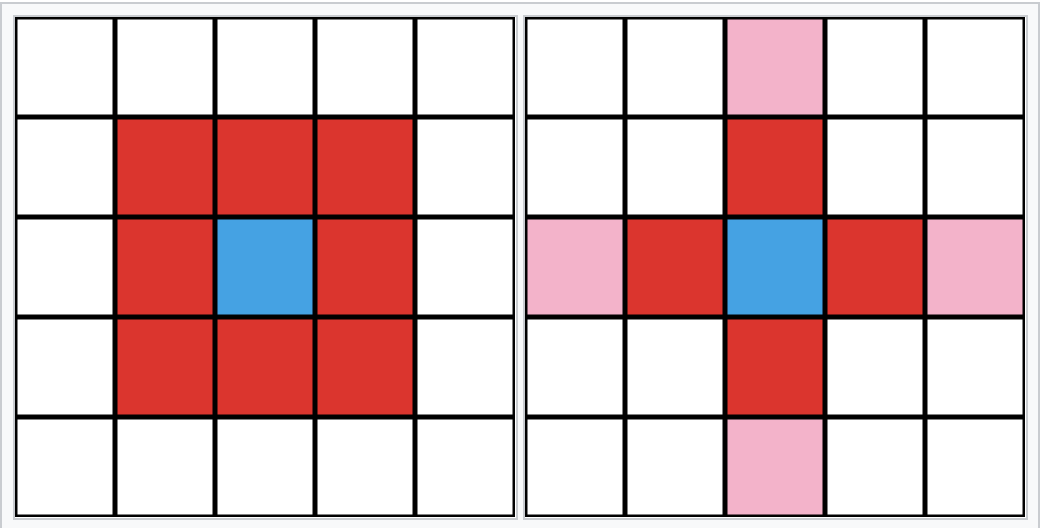
\includegraphics[scale=0.70]{neighbour_differences.png}
\end{figure}
\\
In contrast to the Moore Neigbourhood, the Von Neumann Neighbourhood only considers the adjacently placed cells of a cell in the center. Like the Moore Neighbourhood, the Von-Neumann neighbourhood may also consider the search depth of the neighbours, also defined as the manhattan distance from the center cell. On the right-hand side of the Figure \ref{moore_vs_vn} above, for the Von-Neumann neighbourhood, the red cells are Von-Neumann neighbours of manhattan distance \textit{r} = 1, whereas the pink ones are of \textit{r} = 2.
\\ \\
In terms of changes towards the implementation, the JSON Schema fed to the validator will need to add a required neighbour-type field in the \texttt{conditional\_requirements} property, particularly in the \texttt{reqs\_list} to validate the neighbourhood type. In the actuator component, another function (e.g. \texttt{count\_vn\_neighbours()}) can be written beside the default \texttt{countNeighbours()} (change to perhaps \texttt{count\_m\_neighbours()}). Once these functionalities are implemented, this will allow the function builder component to return a new anonymous function implementing the functionality of the Von-Neumann Neighbourhood. 
\\ \\
Once implemented, the Von-Neumann Neighbourhood may serve as a basic building block of defining the notion of 4-connected pixels in the field of computer graphics \cite{wilson2000handbook}, adding more levels of universality to the simulator.
\newpage

\section{Conclusion and Personal Achievements}
Considering the amount of time that was spent researching and developing for the project, I learned a great deal throughout the entire process. Revisiting HTML and JS was a rewarding experience for me as it has been quite a while since I've developed using those languages. I gained invaluable experience as well, particularly in conducting qualitative interviews to evaluate. Overall, this learning experience was extremely rewarding for me as I got to push my boundaries and nurture my resourcefulness. So many things that I didn't expect to learn by studying Computer Science. This experience and lessons learnt are invaluable, and I will certainly keep pushing my boundaries and abilities as I did from this project's start to finish.

\bibliography{refs}             % this causes the references to be
                                % listed

\bibliographystyle{plain}       % this determines the style in which
                                % the references are printed, other
                                % possible values are plain and abbrv
%% Appendices start here
\appendix
\chapter{Interview Questionnaire}
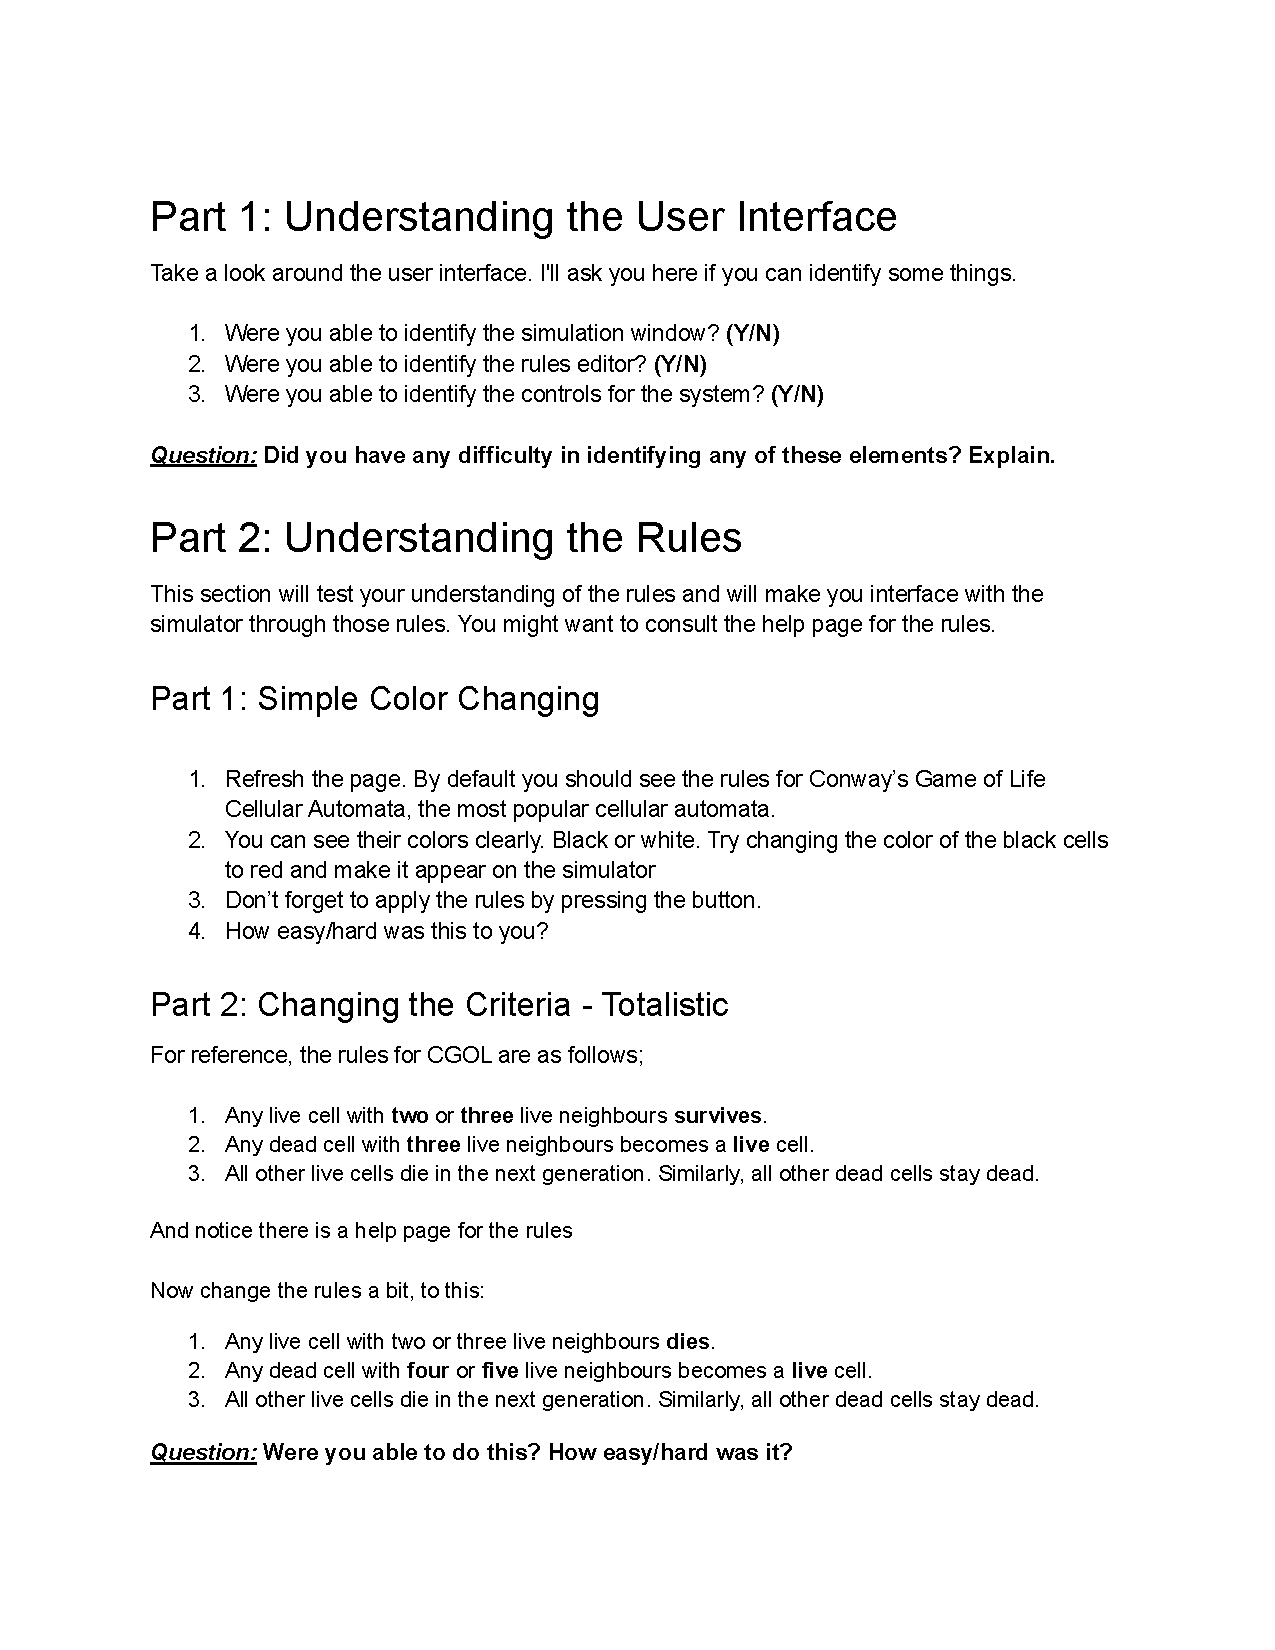
\includepdf[pages=1-2]{resources/interview_qs_project.pdf}
\label{appendix:questionnaire}




% Local Variables: 
% mode: latex
% TeX-master: "report"
% End: 

\chapter{Default Rules}
\label{appendix:default_ca_rules}

\section{Conway's Game of Life}
\label{appendix:default_cgol}
\begin{verbatim}
    {
        "$_meta": {
            "num_states": 2,
            "colors": {
                "0": "black",
                "1": "white"
            }
        },
        "0": {
            "next": {
                "conditional_requirements": [
                    {
                        "type": "totalling",
                        "neighbour_state": 1,
                        "total": [
                            3
                        ]
                    }
                ],
                "satisfied": 1,
                "else": 0
            }
        },
        "default": {
            "next": {
                "conditional_requirements": [
                    {
                        "type": "totalling",
                        "neighbour_state": 1,
                        "total": [
                            2,
                            3
                        ]
                    }
                ],
                "satisfied": 1,
                "else": 0
            }
        }
    }
  
\end{verbatim}

\section{Forest Fire Simulator}
\begin{verbatim}
{
    "$_meta": {
        "num_states": 3,
        "colors": {
            "0": "black",
            "1": "green",
            "2": "red"
        }
    },
    "1": {
        "next": {
            "conditional_requirements": [
                {
                    "type": "total-p",
                    "neighbour_state": 2,
                    "total": [
                        1,
                        2,
                        3,
                        4
                    ],
                    "p": 1
                },
                {
                    "type": "total-p",
                    "neighbour_state": 2,
                    "total": [
                        5, 6, 7, 8
                ],
                    "p": 0.8
                }
            ],
            "satisfied": 2,
            "else": 1
        }
    },
    "default": {
        "next": {
            "conditional_requirements": [
                {
                    "type": "probability",
                    "p": 1
                }
            ],
            "satisfied": 0,
            "else": 0
        }
    }
}

\end{verbatim}

\section{Game Development Map Generation}
\label{appendix:gamedevmap_rules}
\begin{verbatim}
{
    "$_meta": {
        "num_states": 2,
        "colors": {
            "0": "blue",
            "1": "green"
        }
    },
    "default": {
        "next": {
            "conditional_requirements": [
                {
                    "type": "totalling",
                    "neighbour_state": 1,
                    "total": [
                        1, 2, 3, 4
                    ]
                }
            ],
            "satisfied": 0,
            "else": 1
        }
    }
}
  
\end{verbatim}
\chapter{JSON Schema}
\label{appendix:jsonschema}

\begin{verbatim}
    {
    type: "object",
    properties: {
        $_meta: {
            type: "object",
            additionalProperties: false,
            properties: {
                num_states: {
                    type: "integer"
                },
                colors: {
                    type: "object",
                    patternProperties: {
                        "^.*$": {
                            type: "string"
                        }
                    }
                },
            },
            required: ["num_states"]
        },
    },
    patternProperties: {
        "^.*$": {
            $ref: "#/$defs/state",
        },
    },
    $defs: {
        state: {
            type: "object",
            additionalProperties: true,
            properties: {
                next: {
                    type: "object",
                    properties: {
                        conditional_requirements: {
                            $ref: "#/$defs/reqs_list"
                        },
                        satisfied: {
                            type: "integer"
                        },
                        else: {
                            type: "integer"
                        },
                    },
                    required: ["conditional_requirements", "satisfied", "else"],
                },
            },
        },
        reqs_list: {
            type: "array",
            items: [{
                $ref: "#/$defs/reqs"
            }],
        },
        reqs: {
            additionalProperties: true,
            type: "object",
            properties: {
                type: {
                    enum: ["totalling", "total-p", "expression", "probability"],
                },
                neighbour_state: {
                    type: "integer",
                },
                total: {
                    type: "array",
                    items: [{
                        type: "integer"
                    }],
                },
            },
            allOf: [{
                    if: {
                        required: ["type"],
                        properties: {
                            type: {
                                const: "totalling",
                            },
                        },
                    },
                    then: {
                        required: ["neighbour_state", "total"],
                        properties: {
                            neighbour_state: {
                                type: "integer"
                            },
                            total: {
                                type: "array",
                                items: [{
                                    type: "integer",
                                }, ],
                            },
                        },
                    },
                },
                {
                    if: {
                        properties: {
                            type: {
                                const: "total-p",
                            },
                        },
                        required: ["type"],
                    },
                    then: {
                        required: ["neighbour_state", "p", "total"],
                        properties: {
                            neighbour_state: {
                                type: "integer"
                            },
                            p: {
                                type: "number"
                            },
                            total: {
                                type: "array",
                                items: [{
                                    type: "integer",
                                }, ],
                            },
                        },
                    },
                },
                {
                    if: {
                        properties: {
                            type: {
                                const: "expression",
                            },
                        },
                        required: ["type"],
                    },
                    then: {
                        required: ["lhs", "rhs", "cmp"],
                        properties: {
                            lhs: {
                                type: "object",
                                properties: {
                                    neighbour_states: {
                                        type: "array",
                                        items: [{
                                            type: "integer"
                                        }],
                                    },
                                },
                            },
                            rhs: {
                                type: "object",
                                properties: {
                                    neighbour_states: {
                                        type: "array",
                                        items: [{
                                            type: "integer"
                                        }],
                                    },
                                },
                            },
                            cmp: {
                                enum: ["<", ">", "="],
                            },
                        },
                    },
                },
                {
                    if: {
                        properties: {
                            type: {
                                const: "probability",
                            },
                        },
                        required: ["type"],
                    },
                    then: {
                        required: ["p"],
                        properties: {
                            p: {
                                type: "number"
                            },
                        },
                    },
                },
            ],
        },
    },
}
\end{verbatim}

% Local Variables: 
% mode: latex
% TeX-master: "report"
% End: 

\end{document}
